\documentclass[hyperref={pdfpagelabels=false}]{beamer}
% beamer already loads hyperref; do NOT load \usepackage{hyperref} again.

\usepackage{ragged2e} % 文字向兩邊對齊
\renewcommand{\raggedright}{\leftskip=0pt \rightskip=0pt plus 0cm}

\usepackage{listings}
\usepackage{lmodern}
\usepackage{fontspec}
\usepackage{xeCJK}
\setCJKmainfont{Noto Sans CJK TC}
%（可選）若你會用到無襯線中文或等寬中文，建議補上：
\setCJKsansfont{Noto Sans CJK TC}
\setCJKmonofont{Noto Sans Mono CJK TC}

\usepackage[english]{babel}
\usepackage{amsmath,amssymb,amsfonts,amsthm}

% hyperref settings (since beamer already loads hyperref)
\hypersetup{
  colorlinks=true,
  urlcolor=blue,
  citecolor=blue,
  pdfborder={0 0 0}
}

\usepackage{accsupp}% http://ctan.org/pkg/accsupp
\newcommand{\emptyaccsupp}[1]{\BeginAccSupp{ActualText={}}#1\EndAccSupp{}}

\usepackage{tikz}
\usetikzlibrary{arrows,decorations.pathmorphing,backgrounds,fit,positioning,shapes.symbols,chains}

\usepackage{booktabs}
\usepackage{threeparttable}
\usepackage{colortbl} 
\usepackage{xcolor}
\usetikzlibrary{tikzmark}

\newcommand{\indep}{\perp\!\!\!\perp}
\newcommand{\nindep}{\not\!\perp\!\!\!\perp}

\beamertemplatefootpagenumber


\usepackage{listings}
%%%%%%%%%%%%%%%%%%%%%%%%%%%%%%%%%%%%%%%%%%%%%%%%%%%%%%%%%%%%%%%%%%%%%%%%%%%%%%
% LaTeX snippet: language and style definition of Stata for listings package.
%                [listings](http://www.ctan.org/pkg/listings) 
%                [Stata](http://www.stata.com/)
%
% Usage:
%     Copy the code into your preamble, or import it by `\include` .
%     then in your doc:
%     \lstinputlisting[style=numbers]{DO-SCRIPT}
%     \lstinputlisting[style=numbers, style=stata-editor]{DO-SCRIPT}
%     \lstinputlisting[style=nonumbers, frame=none]{DO-SCRIPT}
% How it works:
%     - The language is defined by `\lstdefinelanguage{Stata}`
%     - Four styles is defined by `\lstdefinestyle{STYLE-NAME}`, 
%       they are: numbers and no numbers, plain(black and white) and colorful
%       (colored roughly like stata editor.)
% Tips:
%     - Generally you only need to set your default in the last part,
%       that is, code inside of `\lstset`.
%     - Add more keywords(I can not list all of them) in the `\lstset` part.
%     - Do NOT leave any blank lines in commands
%       (`\lstddefinelanguage', `\lstdefinestyle` and `\lstset`)
%
% update: 2014-04-16
% version: 0.1
% author: kongs
% licence: MIT
% url: https://gist.github.com/kongs-sublime/10862838
%
% TODO: 
%       - finish keyword list.
%       - precise colors that match stata editor?
%       - make it flexible(fonts and style)
%
%%%%%%%%%%%%%%%%%%%%%%%%%%%%%%%%%%%%%%%%%%%%%%%%%%%%%%%%%%%%%%%%%%%%%%%%%%%%%%


% langugae defination
\lstdefinelanguage{Stata}{
	% Left for users to add missing commands,
	% with possibility of choosing different style.
	morekeywords=,
	% Popular add-on commands
	morekeywords=[2]{cntrade, chinafin, 
		wbopendata, spmap,
	},
	% System commands
	morekeywords=[3]{regress, summarize, 
		display,
	},
	% Keywords
	morekeywords=[4]{forvalues, if, foreach, set},
	% Built-in functions
	morekeywords=[5]{rnormal, runiform},
	morecomment=[l]{//},
	% morecomment=[l]{*},  // `*` maybe used as multiply operator. So use `//` as line comment.
	morecomment=[s]{/*}{*/},
	% morecomment=[s]{,}{//},
	% The following is used by macros, like `lags'.
	morecomment=[n][keywordstyle9]{`}{'},
	morestring=[b]",
	sensitive=true,
}

\lstdefinestyle{numbers}{
	numbers=left, 
	stepnumber=1, 
	numberstyle=\tiny\emptyaccsupp,
	xleftmargin=2em,
}

\lstdefinestyle{nonumbers}{
	numbers=none,
}

\lstdefinestyle{stata-plain}{
	language=Stata,
	basicstyle=\footnotesize\ttfamily,
}

\lstdefinestyle{stata-editor}{
	language=Stata,
	basicstyle=\footnotesize\ttfamily,  
	keywordstyle={\color{NavyBlue}},  
	keywordstyle=[2]{\color{NavyBlue}},
	keywordstyle=[3]{\color{NavyBlue}},
	keywordstyle=[4]{\color{NavyBlue}},
	keywordstyle=[5]{\color{Blue}},
	keywordstyle=[9]{\color{TealBlue}},
	stringstyle=\color{Maroon},
	commentstyle=\color{OliveGreen},
}

\lstset{
	language=Stata,
	style=stata-plain,
	% style=stata-editor,
	style=numbers,
	showstringspaces=false,
	breaklines,
	frame=single,
	% To add missing commands
	% morekeywords={xtreg, xtunitroot},
}




\title[] 
{Causal Machine Learning (I): Regression}
%{Regression and Causal Inference}

%\subtitle
%{免除部分負擔對幼兒醫療利用與健康的影響:斷點迴歸分析}

%\author 
 %{Tzu-Ting Yang\inst{1} \and Hsing-Wen Han\inst{2} \and Hsien-Ming Lien\inst{3}}

%\institute[short]{\inst{1} Academia Sinica \and \inst{2} Tamkang University \and \inst{3} National Chengchi University}


\author 
{Prof. Tzu-Ting Yang  \\ 楊子霆}

%\institute{Institute of Economics, Academia Sinica  \\ Econ, NTU}
\institute{Institute of Economics, Academia Sinica  \\ 中央研究院經濟研究所}
%\institute{Institute of Economics, Academia Sinica  \\ Econ, NTU}
%\institute{Institute of Economics, Academia Sinica  \\ IMES/IDAS, NCCU}

%\author 
%{楊子霆 \\ 中研院經濟所}

%\institute 
%{中正大學國際經濟專題研討}




\date
{\today}


% \usetheme{CambridgeUS}
% %\usecolortheme{seahorse}
% \setbeamertemplate{footline}{%
% 	\hfill\usebeamercolor[fg]{page number in head/foot}%
% 	\usebeamerfont{page number in head/foot}%
% 	\insertframenumber\,/\,\inserttotalframenumber\hspace{1em}\vspace{2pt}%
% }

\usetheme{Boadilla}
%\useinnertheme{rectangles}

%\usetheme{CambridgeUS}
\usecolortheme{seahorse}
\setbeamertemplate{footline}{%
	\hfill\usebeamercolor[fg]{page number in head/foot}%
	\usebeamerfont{page number in head/foot}%
	\insertframenumber\,/\,\inserttotalframenumber\hspace{1em}\vspace{2pt}%
}


% \usepackage{beamerthemeshadow}
% %\usecolortheme{seahorse}
% \setbeamertemplate{footline}{%
% 	\hfill\usebeamercolor[fg]{page number in head/foot}%
% 	\usebeamerfont{page number in head/foot}%
% 	\insertframenumber\,/\,\inserttotalframenumber\hspace{1em}\vspace{2pt}%
% }


%\usepackage{beamerthemeshadow}

\beamersetuncovermixins{\opaqueness<1>{25}}{\opaqueness<2->{15}}

\begin{document}


\begin{frame}{}
 \titlepage
\end{frame}







\title[]
{Main Idea}


\author
{}

%\institute{Institute of Economics, Academia Sinica  \\ Econ, NTU}
%\institute{Institute of Economics, Academia Sinica  \\ IMES/IDAS, NCCU}
\institute{}

%\author
%{楊子霆 \\ 中研院經濟所}

%\institute
%{中正大學國際經濟專題研討}




\date
{}


\begin{frame}{}
	\titlepage
\end{frame}




\begin{frame}{Causal Machine Learning: Overview}
	\begin{itemize}
		\item \textbf{Machine learning (ML)} methods use data-driven algorithms to model the relationship between an outcome \textbf{Y} and covariates \textbf{X}
		\vspace{0.2cm}
		\begin{itemize}
			\item There are many ML methods; \textbf{regression} is a fundamental one
			\vspace{0.2cm}
			\item The best method depends on the application
		\end{itemize}
		\vspace{0.3cm}
		\item For \textbf{causal inference}, ML methods help us select and control for relevant covariates, enabling credible identification of treatment effects
		\vspace{0.3cm}
		\item This lecture series covers three approaches:
		\vspace{0.2cm}
		\begin{itemize}
			\item \textbf{Part I (This Lecture):} Regression --- the foundational ML tool for causal inference under selection on observables
			\vspace{0.2cm}
			\item \textbf{Part II:} Post-Double Selection --- handling high-dimensional covariates with LASSO
			\vspace{0.2cm}
			\item \textbf{Part III:} Heterogeneous Treatment Effects --- estimating CATE with Causal Forest
		\end{itemize}
	\end{itemize}
\end{frame}







\begin{frame}{Machine Learning as a Prediction Tool}
	\begin{itemize}
		\item The primary goal of \textbf{machine learning} is to \textbf{predict} an outcome $Y$ given covariates $X$
		\vspace{0.2cm}
		\begin{itemize}
			\item \textbf{Regression:} predict a continuous outcome (e.g., wages, earnings)
			\vspace{0.2cm}
			\item \textbf{Classification:} predict a discrete category (e.g., employed vs. unemployed)
			\vspace{0.2cm}
			\item Classification is also a prediction task --- predict which category a unit belongs to
		\end{itemize}
		\vspace{0.3cm}
		\item ML methods are evaluated by \textbf{out-of-sample prediction accuracy}
		\vspace{0.2cm}
		\begin{itemize}
			\item Minimize prediction error on data not used for estimation
			\vspace{0.2cm}
			\item This is different from the classical econometrics focus on unbiasedness and consistency
		\end{itemize}
		\vspace{0.3cm}
		\item \textbf{Key question:} Can these prediction tools be used for \textbf{causal inference}?
	\end{itemize}
\end{frame}




\begin{frame}{From Prediction to Counterfactual Prediction}
	\begin{itemize}
		\item \textbf{Causal inference} requires answering a fundamentally different question:
		\vspace{0.2cm}
		\begin{itemize}
			\item Not just ``what is $Y$ likely to be given $X$?''
			\vspace{0.2cm}
			\item But ``what would $Y$ have been \textbf{under a different treatment status}?'' $\longrightarrow$ \textbf{counterfactual}
		\end{itemize}
		\vspace{0.3cm}
		\item \textbf{Fundamental Problem of Causal Inference:} We only observe one potential outcome per individual
		\vspace{0.2cm}
		\begin{itemize}
			\item For treated units ($D_i=1$): observe $Y^{1}_i$, but not $Y^{0}_i$
			\vspace{0.2cm}
			\item For untreated units ($D_i=0$): observe $Y^{0}_i$, but not $Y^{1}_i$
		\end{itemize}
		\vspace{0.3cm}
		\item \textbf{ML methods help us predict the missing counterfactual:}
		\vspace{0.2cm}
		\begin{itemize}
			\item Use $X_i$ to find units with similar characteristics but different treatment status
			\vspace{0.2cm}
			\item Under the right assumptions (CIA), the predicted counterfactual is valid
			\vspace{0.2cm}
			\item \textbf{Regression} is the simplest ML tool for predicting counterfactual outcomes
		\end{itemize}
	\end{itemize}
\end{frame}




\begin{frame}{Main Idea of Regression}
	\begin{itemize}
		%\item Regression is a way to control observable covariates
		%\vspace{0.3cm}

		\item A multivariate regression can help us study the relationship between treatment $D_i$ and outcome $\mathrm{Y}_i$
		
		
		\begin{equation*}
		\begin{aligned}
		\mathrm{Y}_i &= \delta + \alpha D_i + X_{i} \beta + \epsilon_{i}
		\end{aligned}
		\end{equation*}	
		
		
		\item Here, $X$ is a vector of covariates and  $\beta$ is a vector of coefficients
					\vspace{0.2cm} 
			\begin{itemize}
		\item[] \[ X = (x_1', x_2', \ldots, x_k') \]
					%\vspace{0.2cm} 
	\item[]	\[ \beta = (\beta_1, \beta_2, \ldots, \beta_k) \]
	
	\item[] \[ X \beta = \beta_1 x_1 + \beta_2 x_2 + \cdots + \beta_k x_k \]
				
			\end{itemize}
		

		
		
	\end{itemize}
\end{frame}





\begin{frame}{Main Idea of Regression}
	\begin{itemize}
		\item We can interpret $\alpha$ as the causal effect of treatment when we include all relevant confounding factors $X_{i}$ in the regression
		\vspace{0.2cm}
		\item The inclusion of $X$ allows for an "apples-to-apples" comparison
		\vspace{0.2cm}
		\begin{itemize}
			\item We compare units with the same values of $X$ but different values of treatment $D$
			\vspace{0.2cm}
			%\item This comparison is only valid if $X$ contains all relevant confounding factors
			%\vspace{0.2cm}
		%	\item This causal interpretation relies on the Conditional Independence Assumption (CIA): $(\mathrm{Y}^{1}_{i},\mathrm{Y}^{0}_{i})\indep D_{i}|X_{i}$
		\end{itemize}
	\end{itemize}
\end{frame}














\title[]  
{Identification}


\author 
{}

%\institute{Institute of Economics, Academia Sinica  \\ Econ, NTU}
%\institute{Institute of Economics, Academia Sinica  \\ IMES/IDAS, NCCU}
\institute{}

%\author 
%{楊子霆 \\ 中研院經濟所}

%\institute 
%{中正大學國際經濟專題研討}




\date
{}


\begin{frame}{}
	\titlepage
\end{frame}




\begin{frame}{Identification Assumption}
	
	\begin{block}{Conditional Independence Assumption}
		\begin{equation*}
		(\mathrm{Y}^{1}_{i},\mathrm{Y}^{0}_{i})\indep D_{i}|X_{i}
		\end{equation*}
	\end{block}
	\begin{itemize}
		
		\vspace{0.3cm}
		\item Both matching and regression require CIA (selection on observable) to get causal affects
		\vspace{0.3cm}
		\begin{itemize}
			\item But regression implicitly assume a specific functional form of \textbf{potential outcomes}
			\vspace{0.2cm}
			\item Matching additionally requires \textbf{common support}: treated and control units must overlap in their covariate distributions
			\vspace{0.2cm}
			\item Regression does \textbf{not} require common support --- it extrapolates outside the region of overlap using the assumed functional form
		\end{itemize}
	\end{itemize}
\end{frame}


% \begin{frame}{CIA: What It Implies}
% 	\begin{itemize}
% 		\item Under CIA, treatment assignment is \textbf{as good as random} after conditioning on $X_i$
% 		\vspace{0.3cm}
% 		\item CIA implies that \textbf{selection bias is eliminated} within cells of $X$:
% 		\vspace{0.2cm}
% 		\begin{itemize}
% 			\item $\mathrm{E}[\mathrm{Y}^{0}_{i}\mid X_{i}, D_i=1] = \mathrm{E}[\mathrm{Y}^{0}_{i}\mid X_{i}, D_i=0]$
% 			\vspace{0.2cm}
% 			\item $\mathrm{E}[\mathrm{Y}^{1}_{i}\mid X_{i}, D_i=1] = \mathrm{E}[\mathrm{Y}^{1}_{i}\mid X_{i}, D_i=0]$
% 		\end{itemize}
% 		\vspace{0.3cm}
% 		\item This means treated and control units with the same $X_i$ are \textbf{comparable}:
% 		\vspace{0.2cm}
% 		\begin{itemize}
% 			\item We can use control units' observed $Y^0$ to predict the counterfactual $Y^0$ for treated units
% 			\vspace{0.2cm}
% 			\item We can use treated units' observed $Y^1$ to predict the counterfactual $Y^1$ for control units
% 		\end{itemize}
% 		\vspace{0.3cm}
% 		\item Both matching and regression rely on CIA to get causal effects
% 		\vspace{0.2cm}
% 		\begin{itemize}
% 			\item Regression additionally imposes a specific \textbf{functional form} on potential outcomes
% 		\end{itemize}
% 	\end{itemize}
% \end{frame}









\begin{frame}{Regression and Potential Outcome}
	\begin{itemize}
		\item Regression estimates the causal effect by \textbf{predicting both potential outcomes} and taking the difference
		\vspace{0.2cm}
		\item Under the CIA, we can estimate the following regression to get causal effect of $D$ by including all possible confounding factors $X$
		\begin{equation*}
			\mathrm{Y}_i = \delta + \alpha D_i + X_{i}\beta + \epsilon_{i}
		\end{equation*}
		\item The fitted model predicts \textbf{both} potential outcomes for any unit with covariates $X_i$:
		\vspace{0.1cm}
		\begin{itemize}
			\item Predicted $\mathrm{Y}^{1}$ (set $D=1$): $\quad\mathrm{E}[\mathrm{Y}^{1}_{i}|X_{i}] = \delta + \alpha + X_{i}\beta$
			\vspace{0.15cm}
			\item Predicted $\mathrm{Y}^{0}$ (set $D=0$): $\quad\mathrm{E}[\mathrm{Y}^{0}_{i}|X_{i}] = \delta + X_{i}\beta$
			\vspace{0.15cm}
			\item CIA implies $\mathrm{E}[\epsilon_{i}|D_i,X_{i}] = 0$, so these predictions are valid
		\end{itemize}
		\vspace{0.2cm}
		\item The \textbf{causal effect} is the difference between the two predicted outcomes:
		\begin{equation*}
			\mathrm{E}[\mathrm{Y}^{1}_{i} - \mathrm{Y}^{0}_{i}|X_{i}] = \alpha \quad \text{(constant across all } X_i\text{)}
		\end{equation*}
		%\item Note: Regression imposes a \textbf{constant treatment effect} --- $\alpha$ is the same for everyone
	\end{itemize}
\end{frame}



\begin{frame}{Regression and Matching}{A Graphical Example}
	\begin{itemize}
		
		\item Suppose we want to examine the effect of a treatment $D$ on an outcome $Y$ 
				\vspace{0.2cm}
			\begin{itemize}
		\item Education is a observed confounding factor $X$
						\vspace{0.2cm}
				\end{itemize}
\item Matching:
						\vspace{0.2cm}
\begin{itemize}
	\item Require sufficient overlap in covariate distributions ($X$) between treated and control groups
							\vspace{0.2cm}
	\item This is known as the common support assumption
							\vspace{0.2cm}
	\item Ensures valid counterfactual comparisons
							\vspace{0.2cm}
\end{itemize}


		

	
		
		
	\end{itemize}
\end{frame}



\begin{frame}{Regression and Matching}{A Graphical Example}
	\begin{center}
		\begin{figure}[p]
			\centering
		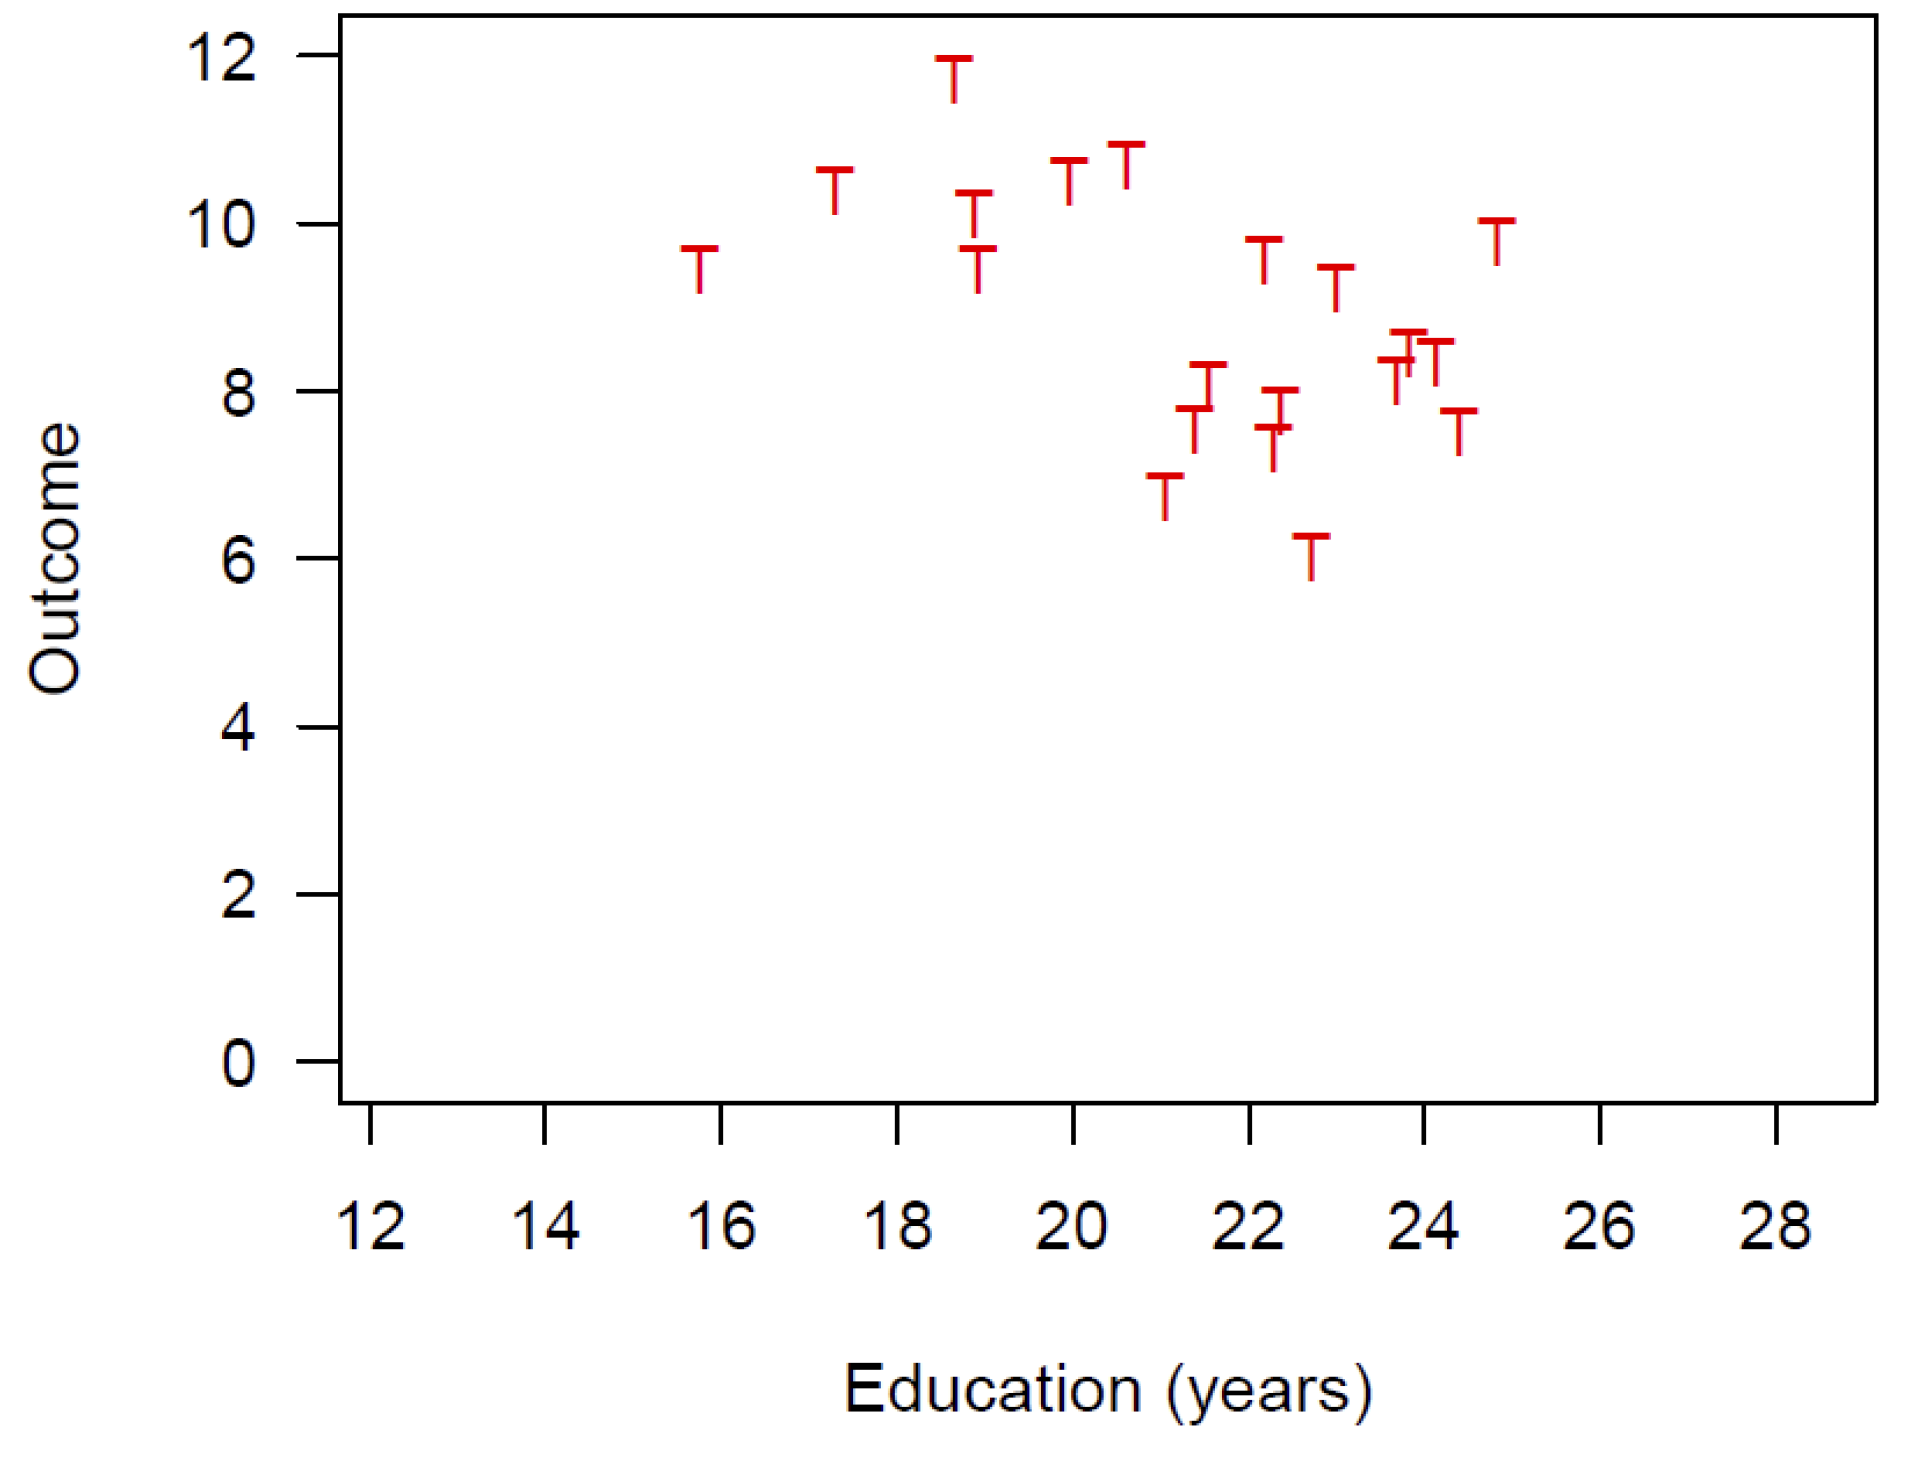
\includegraphics[width=0.7\textwidth]{figure/reg_f1.png}
		\end{figure}
		\begin{minipage}{0.9\linewidth}
			\fontsize{8}{8pt}\selectfont
			\emph{Source:} Ben Elsner's slides
		\end{minipage}
	\end{center}
	
	
\end{frame}


\begin{frame}{Regression and Matching}{A Graphical Example}
		\begin{center}
		\begin{figure}[p]
			\centering
			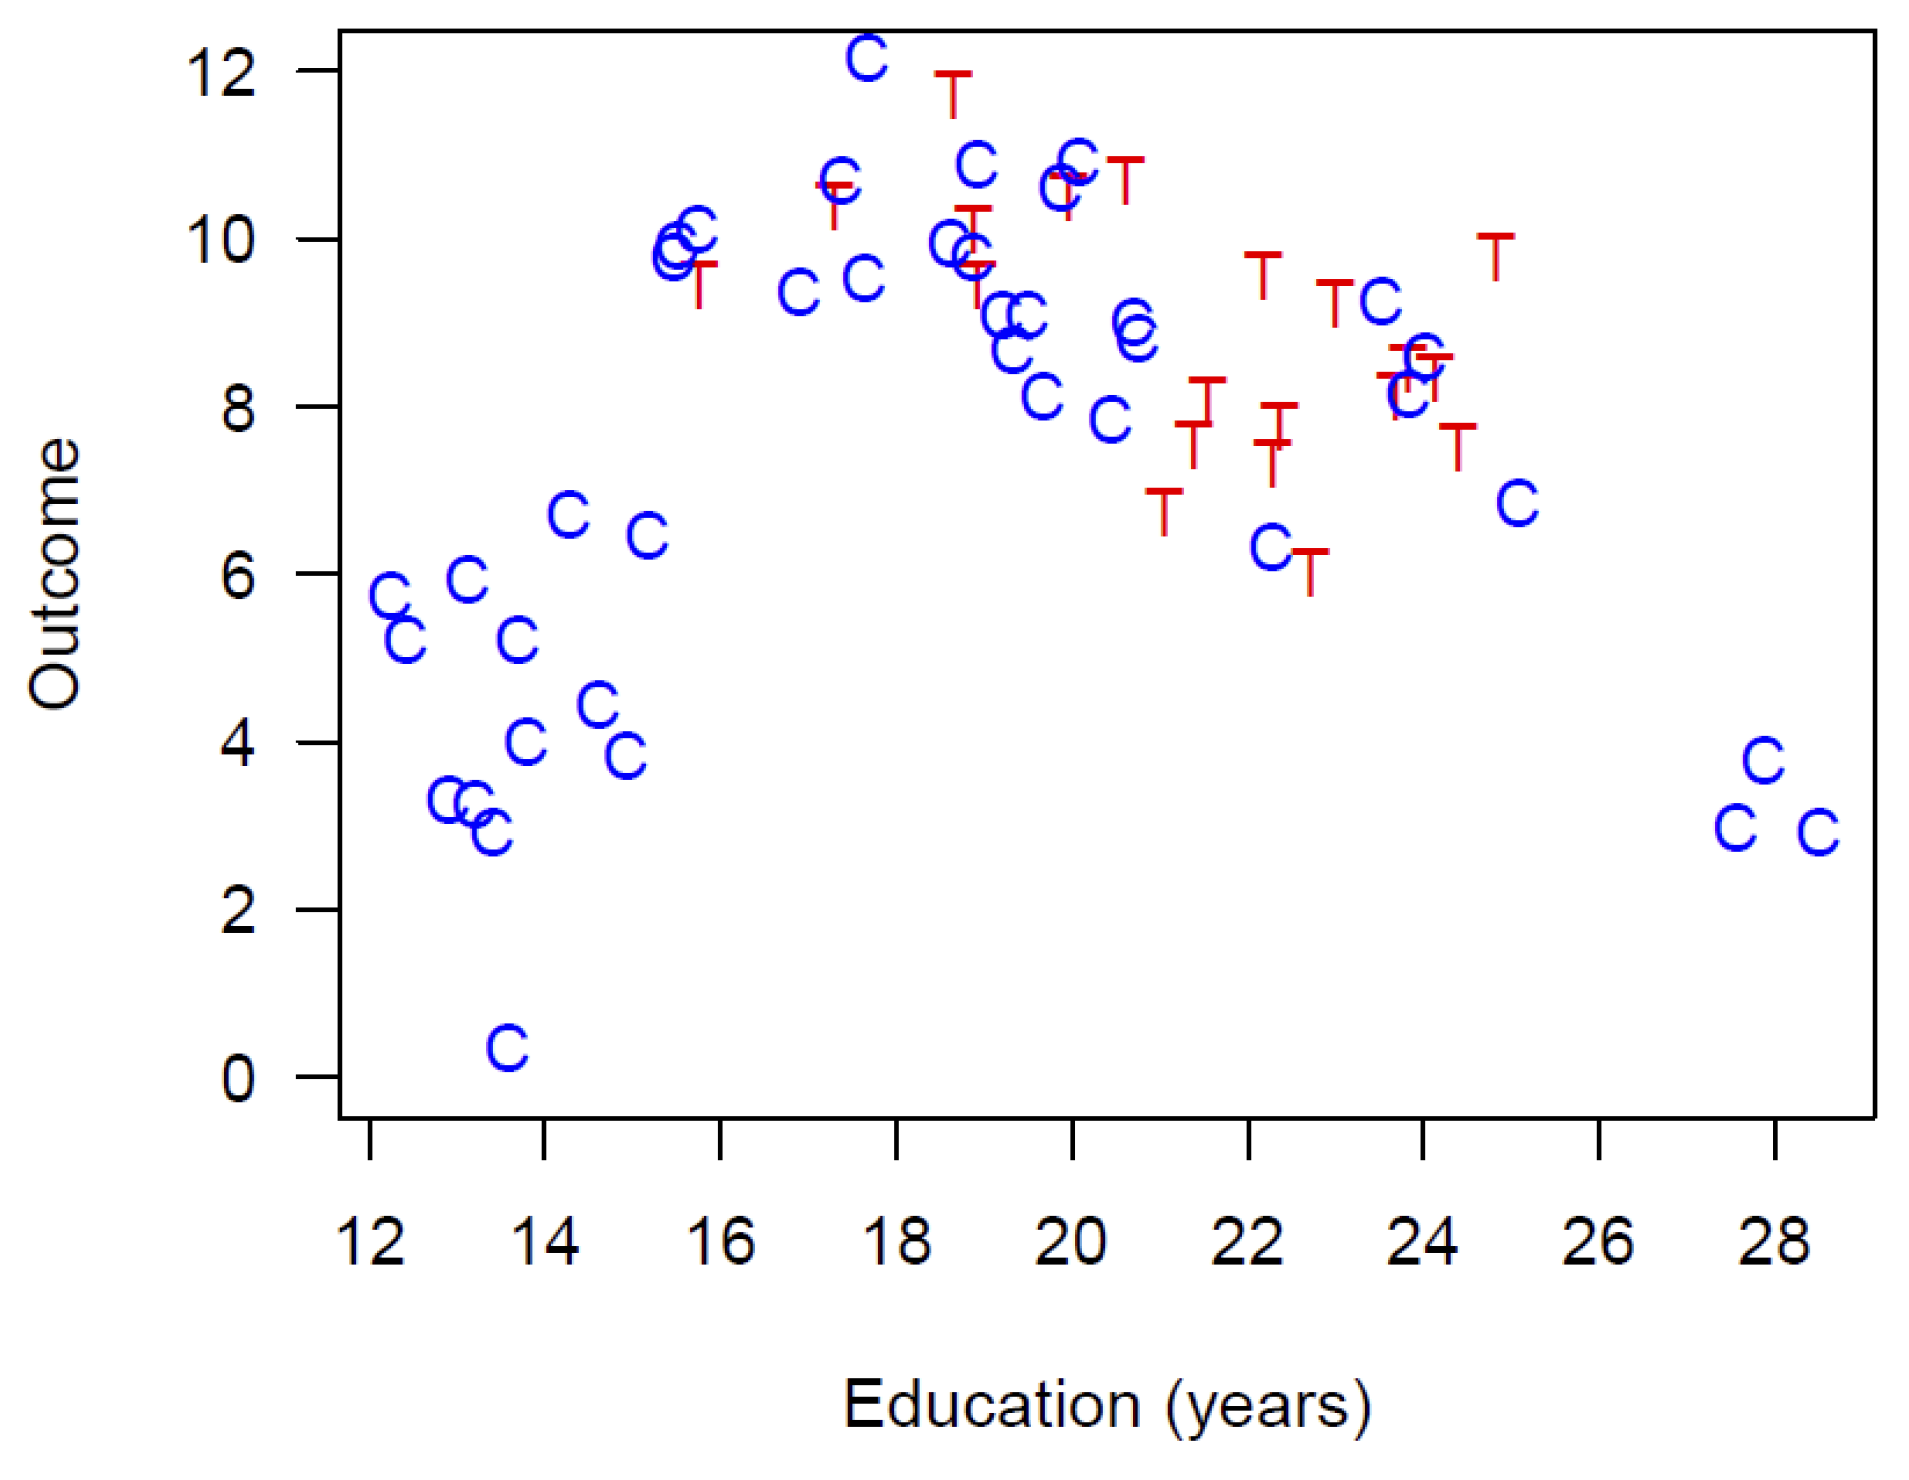
\includegraphics[width=0.7\textwidth]{figure/reg_f2.png}
		\end{figure}
		\begin{minipage}{0.9\linewidth}
			\fontsize{8}{8pt}\selectfont
			\emph{Source:} Ben Elsner's slides
		\end{minipage}
	\end{center}
\end{frame}




\begin{frame}{Regression and Matching}{A Graphical Example}
	\begin{center}
		\begin{figure}[p]
			\centering
			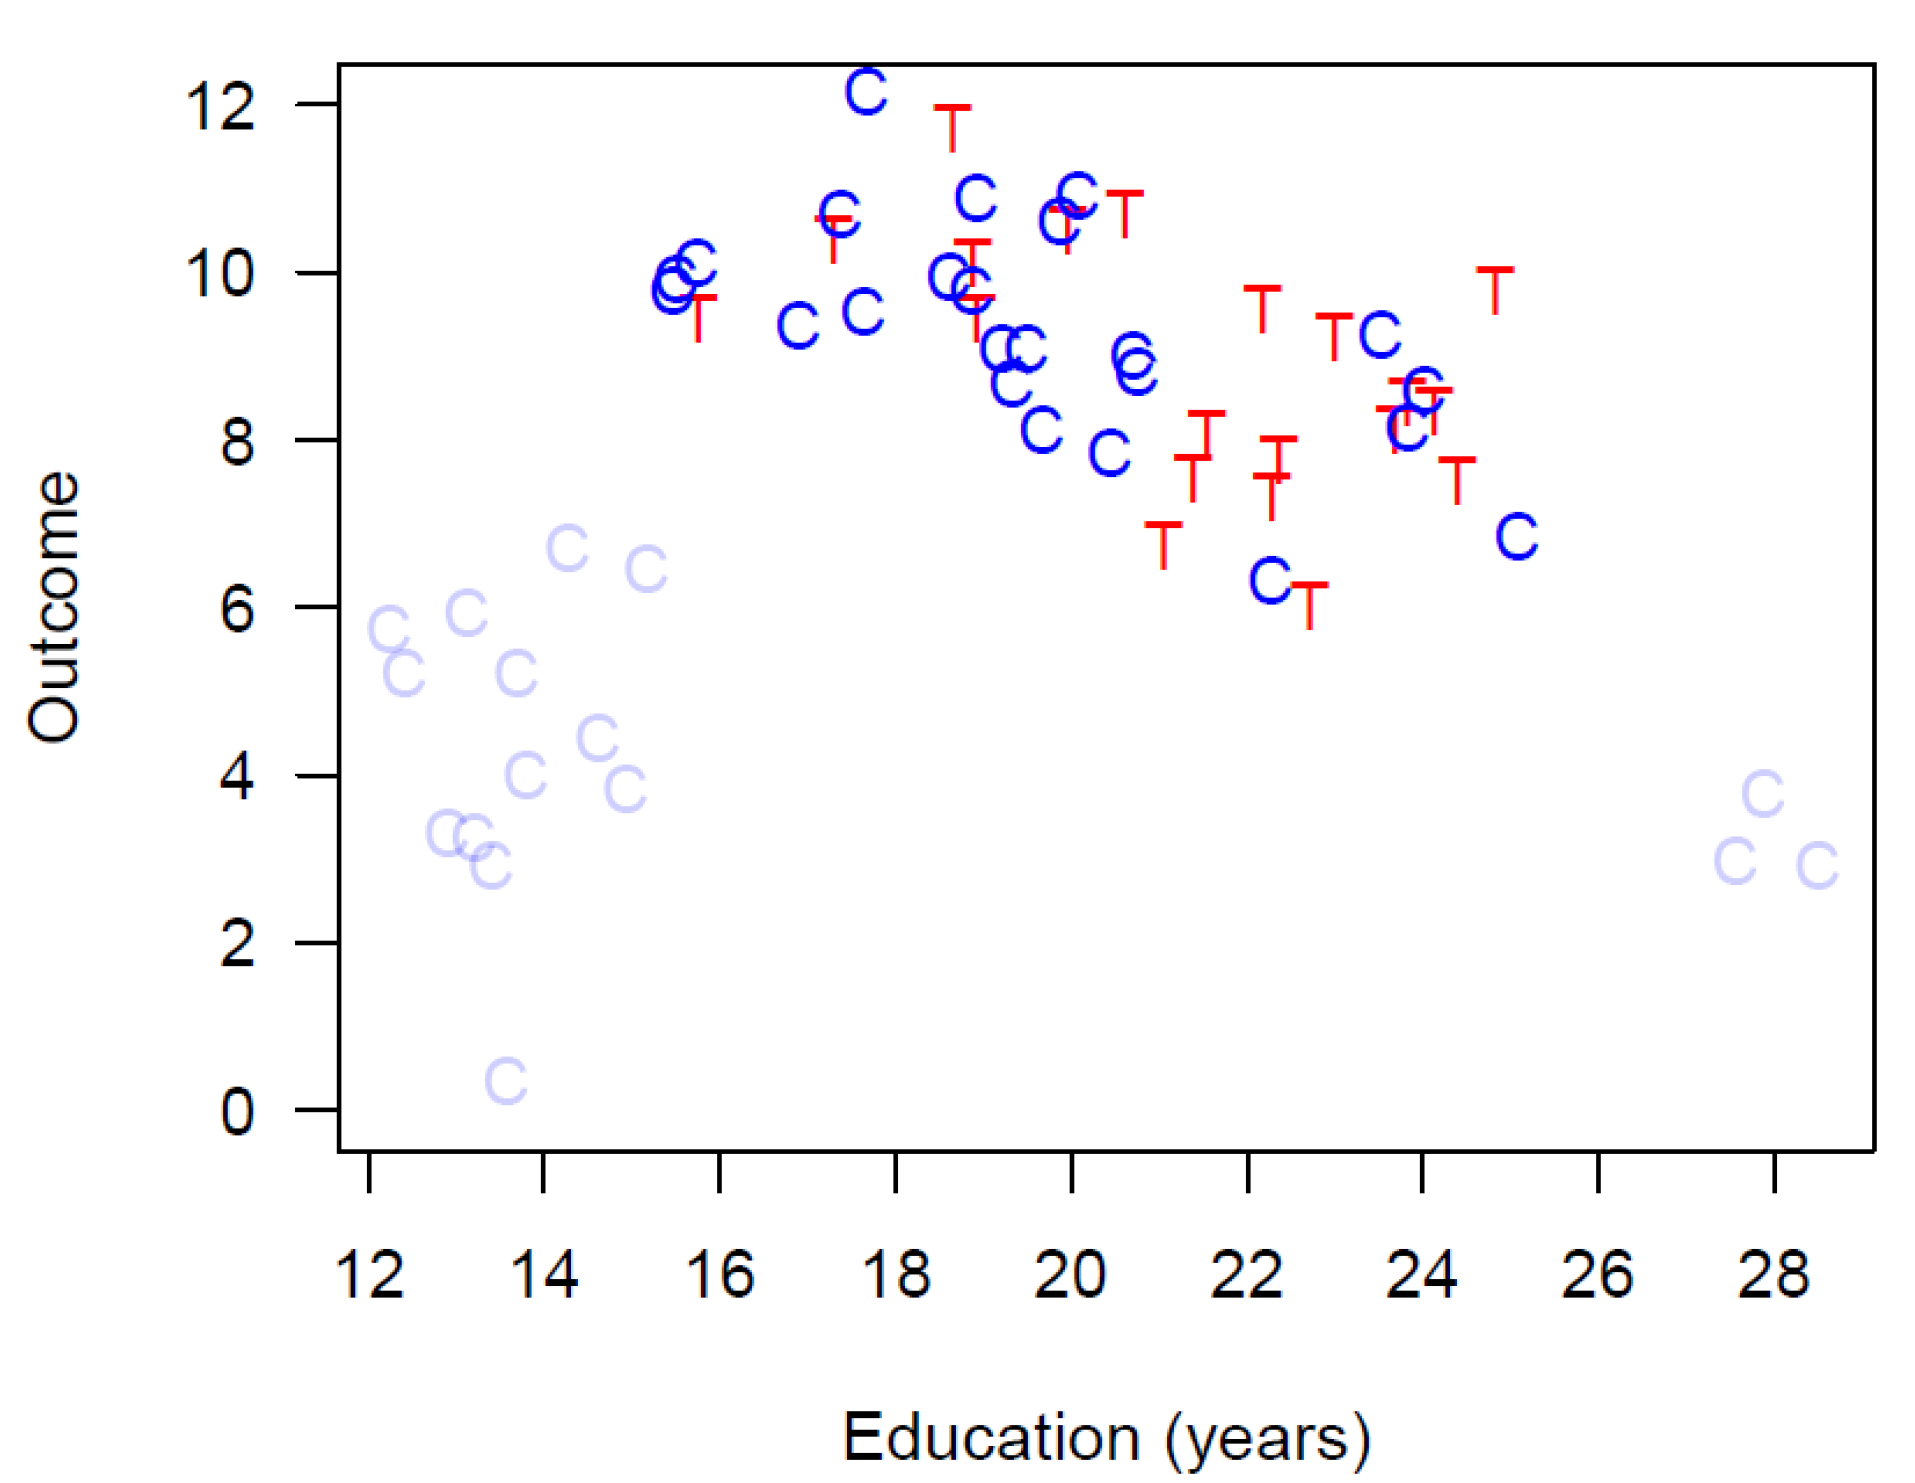
\includegraphics[width=0.7\textwidth]{figure/reg_f5.png}
		\end{figure}
		\begin{minipage}{0.9\linewidth}
			\fontsize{8}{8pt}\selectfont
			\emph{Source:} Ben Elsner's slides
		\end{minipage}
	\end{center}
\end{frame}



\begin{frame}{Regression and Matching}{A Graphical Example}
	\begin{itemize}
		\item Regression:
		\vspace{0.2cm}
		\begin{itemize}
			\item Can potentially extrapolate beyond the common support region
			\vspace{0.2cm}
			\item By relying on the specified regression model to predict counterfactual outcomes
			\vspace{0.2cm}
			\begin{itemize}
				\item Linear term for education: $\mathrm{Y}_{i}= \delta +  \alpha D_i + \beta_{1} X_{i} + \epsilon_{i} $
				\vspace{0.2cm}
				\item Quadratic term for education: $\mathrm{Y}_{i}= \delta +  \alpha D_i + \beta_{1} X_{i} + \beta_{2} X^{2}_{i} + \epsilon_{i} $
				\vspace{0.2cm}	
				\item Estimated effect of treatment $D$ can be different for these two models
				\vspace{0.2cm}								
			\end{itemize}
			\item The extrapolation may be unreliable if:
			\vspace{0.2cm}
			\begin{itemize}
				\item Model is misspecified
				\vspace{0.2cm}
				\item Extrapolation region is too far from data
			\end{itemize}
		\end{itemize}
	\end{itemize}
\end{frame}

\begin{frame}{Regression and Matching}{A Graphical Example}
	\begin{center}
	\begin{figure}[p]
		\centering
		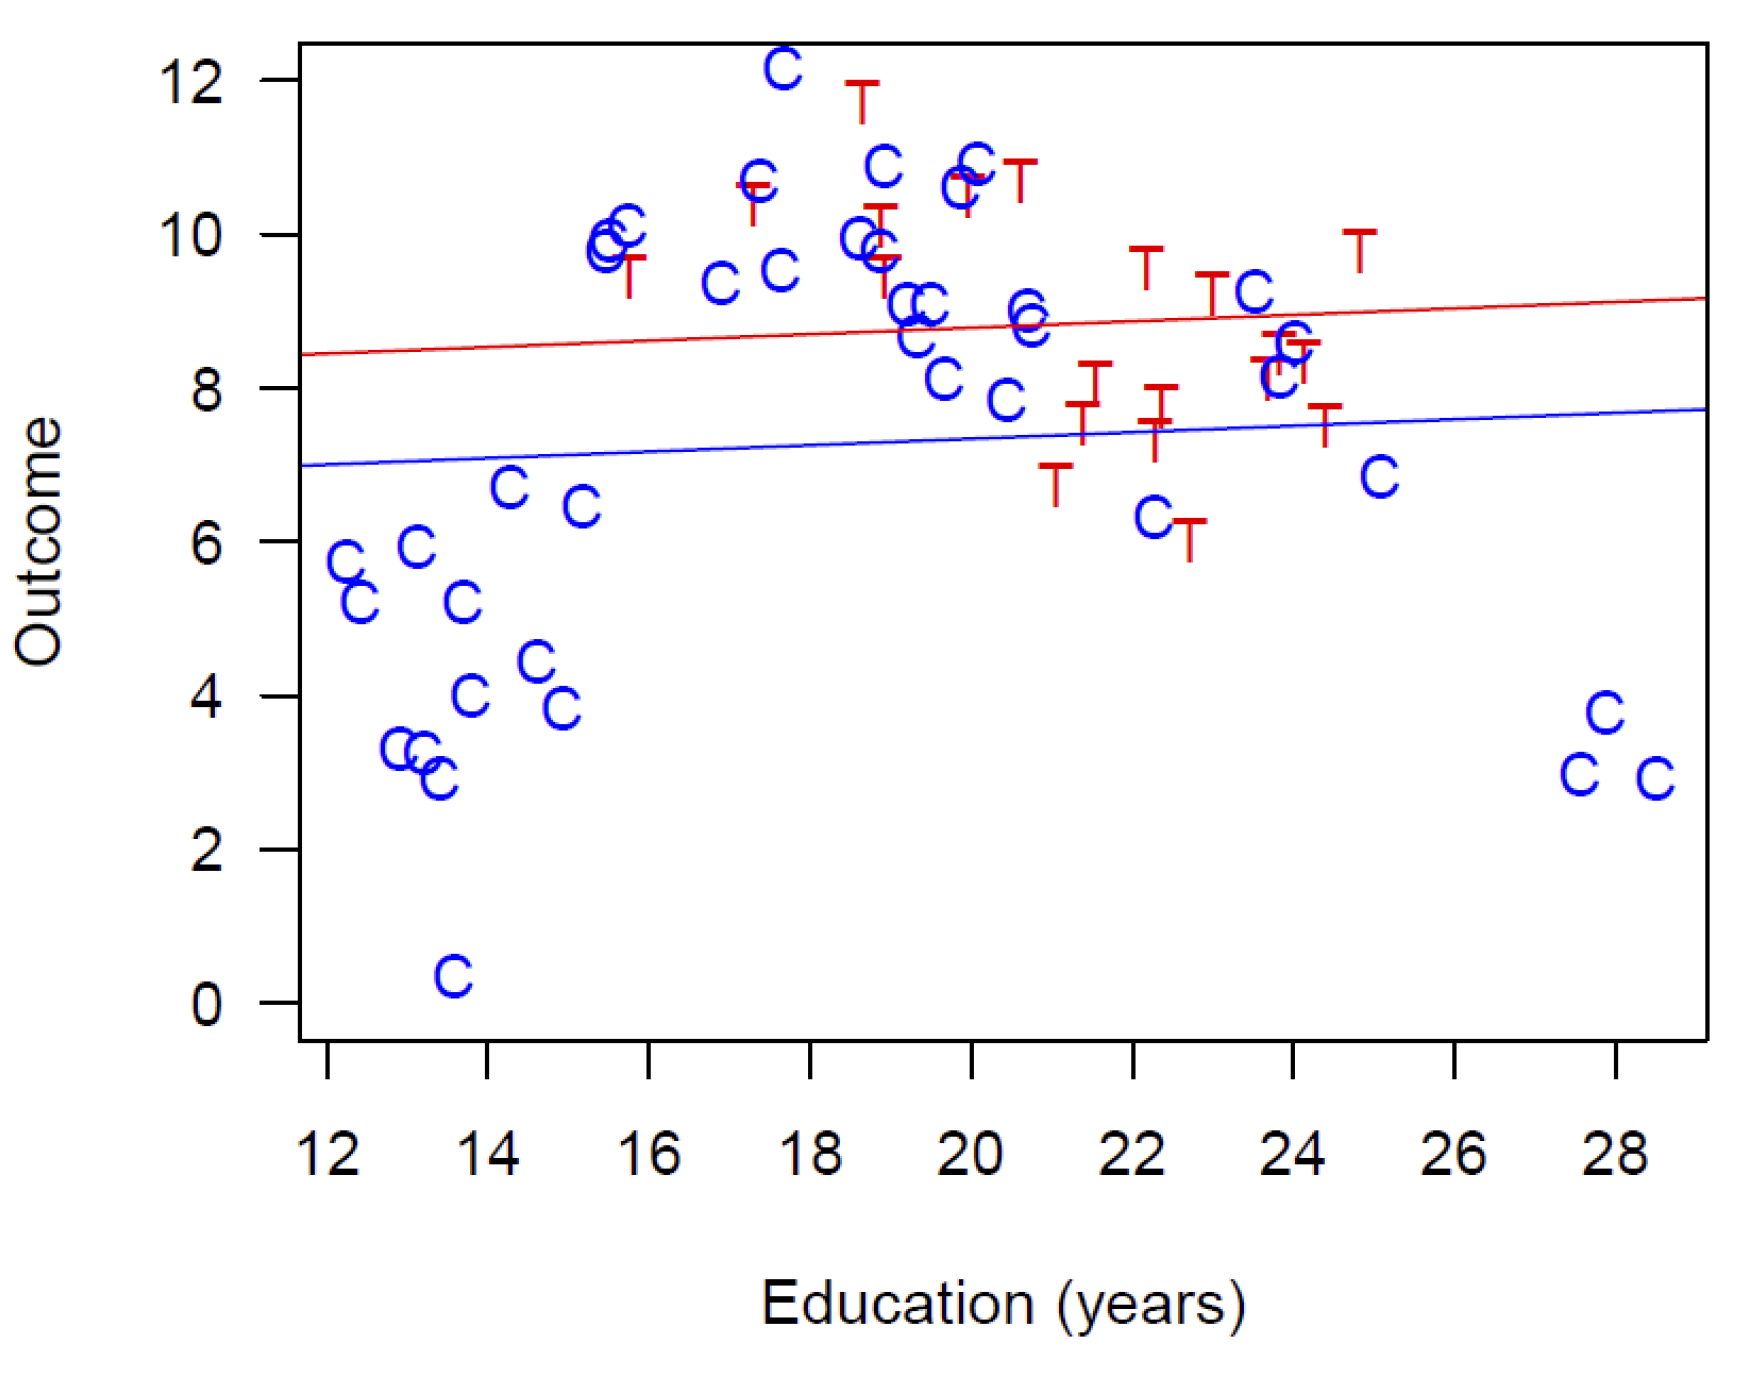
\includegraphics[width=0.7\textwidth]{figure/reg_f3.png}
	\end{figure}
	\begin{minipage}{0.9\linewidth}
		\fontsize{8}{8pt}\selectfont
		\emph{Source:} Ben Elsner's slides
	\end{minipage}
\end{center}
\end{frame}

\begin{frame}{Regression and Matching}{A Graphical Example}
	\begin{itemize}
		\item The \textbf{red line} is the fitted regression for the treated group ($D=1$); the \textbf{blue line} for the control group ($D=0$)
		\vspace{0.3cm}
		\begin{itemize}
			\item Under the linear model, both lines have the \textbf{same slope} ($\beta_1$) but different intercepts
			\vspace{0.2cm}
			\item The \textbf{vertical gap} between the two lines is the estimated treatment effect $\hat{\alpha}$ --- constant across all values of $X$
			% \vspace{0.2cm}
			% \item Even under the linear model, the two lines are extrapolated beyond the common support region --- the gap at any given $X$ relies on the assumed functional form, not just within-support comparisons
		\end{itemize}
	\end{itemize}
\end{frame}

\begin{frame}{Regression and Matching}{A Graphical Example}
	\begin{center}
	\begin{figure}[p]
		\centering
		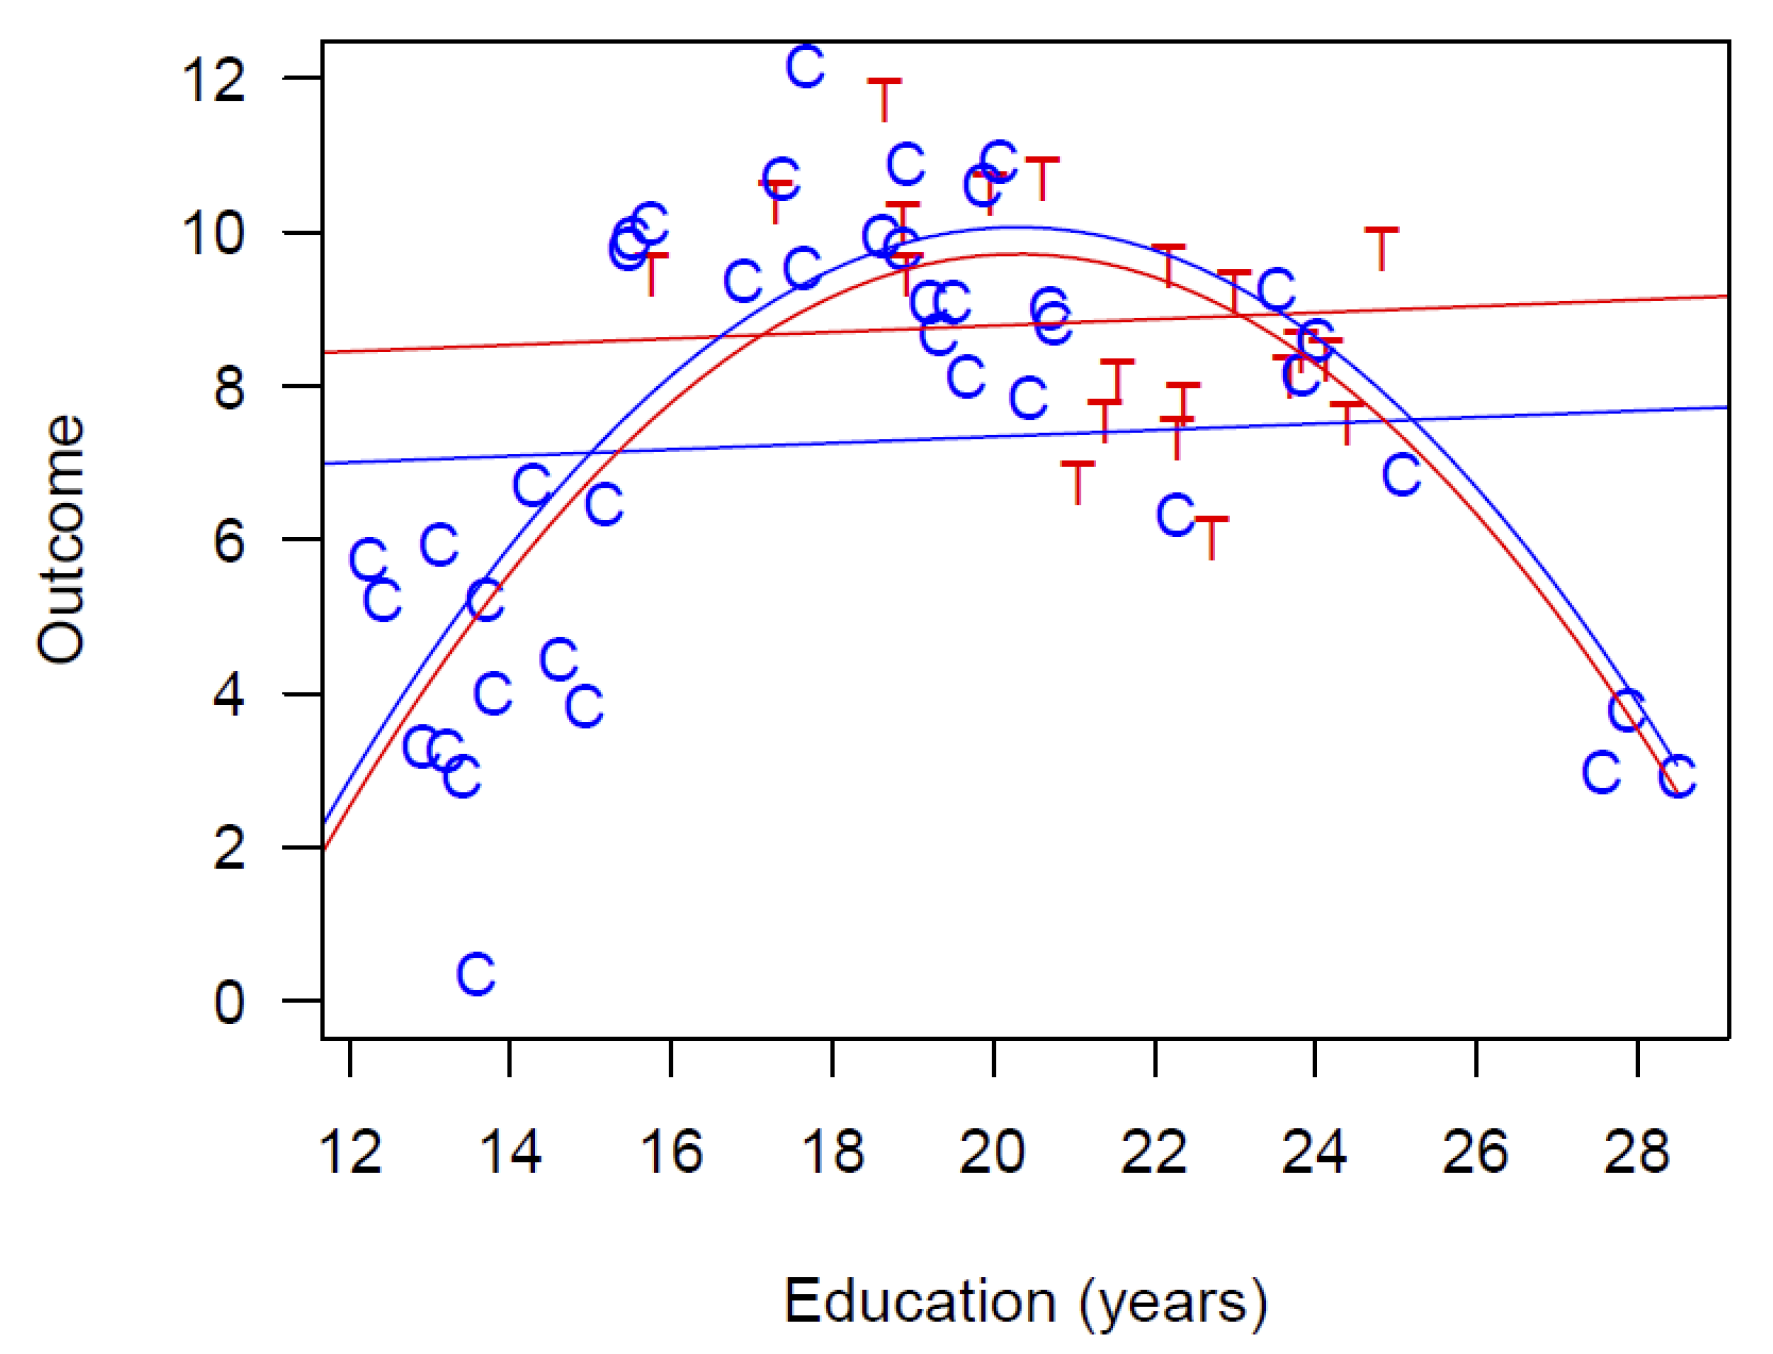
\includegraphics[width=0.7\textwidth]{figure/reg_f4.png}
	\end{figure}
	\begin{minipage}{0.9\linewidth}
		\fontsize{8}{8pt}\selectfont
		\emph{Source:} Ben Elsner's slides
	\end{minipage}
\end{center}
\end{frame}

\begin{frame}{Regression and Matching}{A Graphical Example}
	\begin{itemize}
		\item With a \textbf{quadratic} functional form, the two curves have the same shape but are shifted vertically by $\hat{\alpha}$
		\vspace{0.3cm}
		\begin{itemize}
			\item The vertical gap between the red and blue curves is still the constant treatment effect $\hat{\alpha}$
			\vspace{0.2cm}
			\item However, the \textbf{curvature} of the fitted lines changes how each line extrapolates outside the common support region
			\vspace{0.2cm}
			\item This illustrates why the choice of functional form matters: \alert{different models can yield different treatment effect estimates}
		\end{itemize}
	\end{itemize}
\end{frame}



\begin{frame}{Regression and Matching}{A Graphical Example}
	\begin{center}
		\begin{figure}[p]
			\centering
			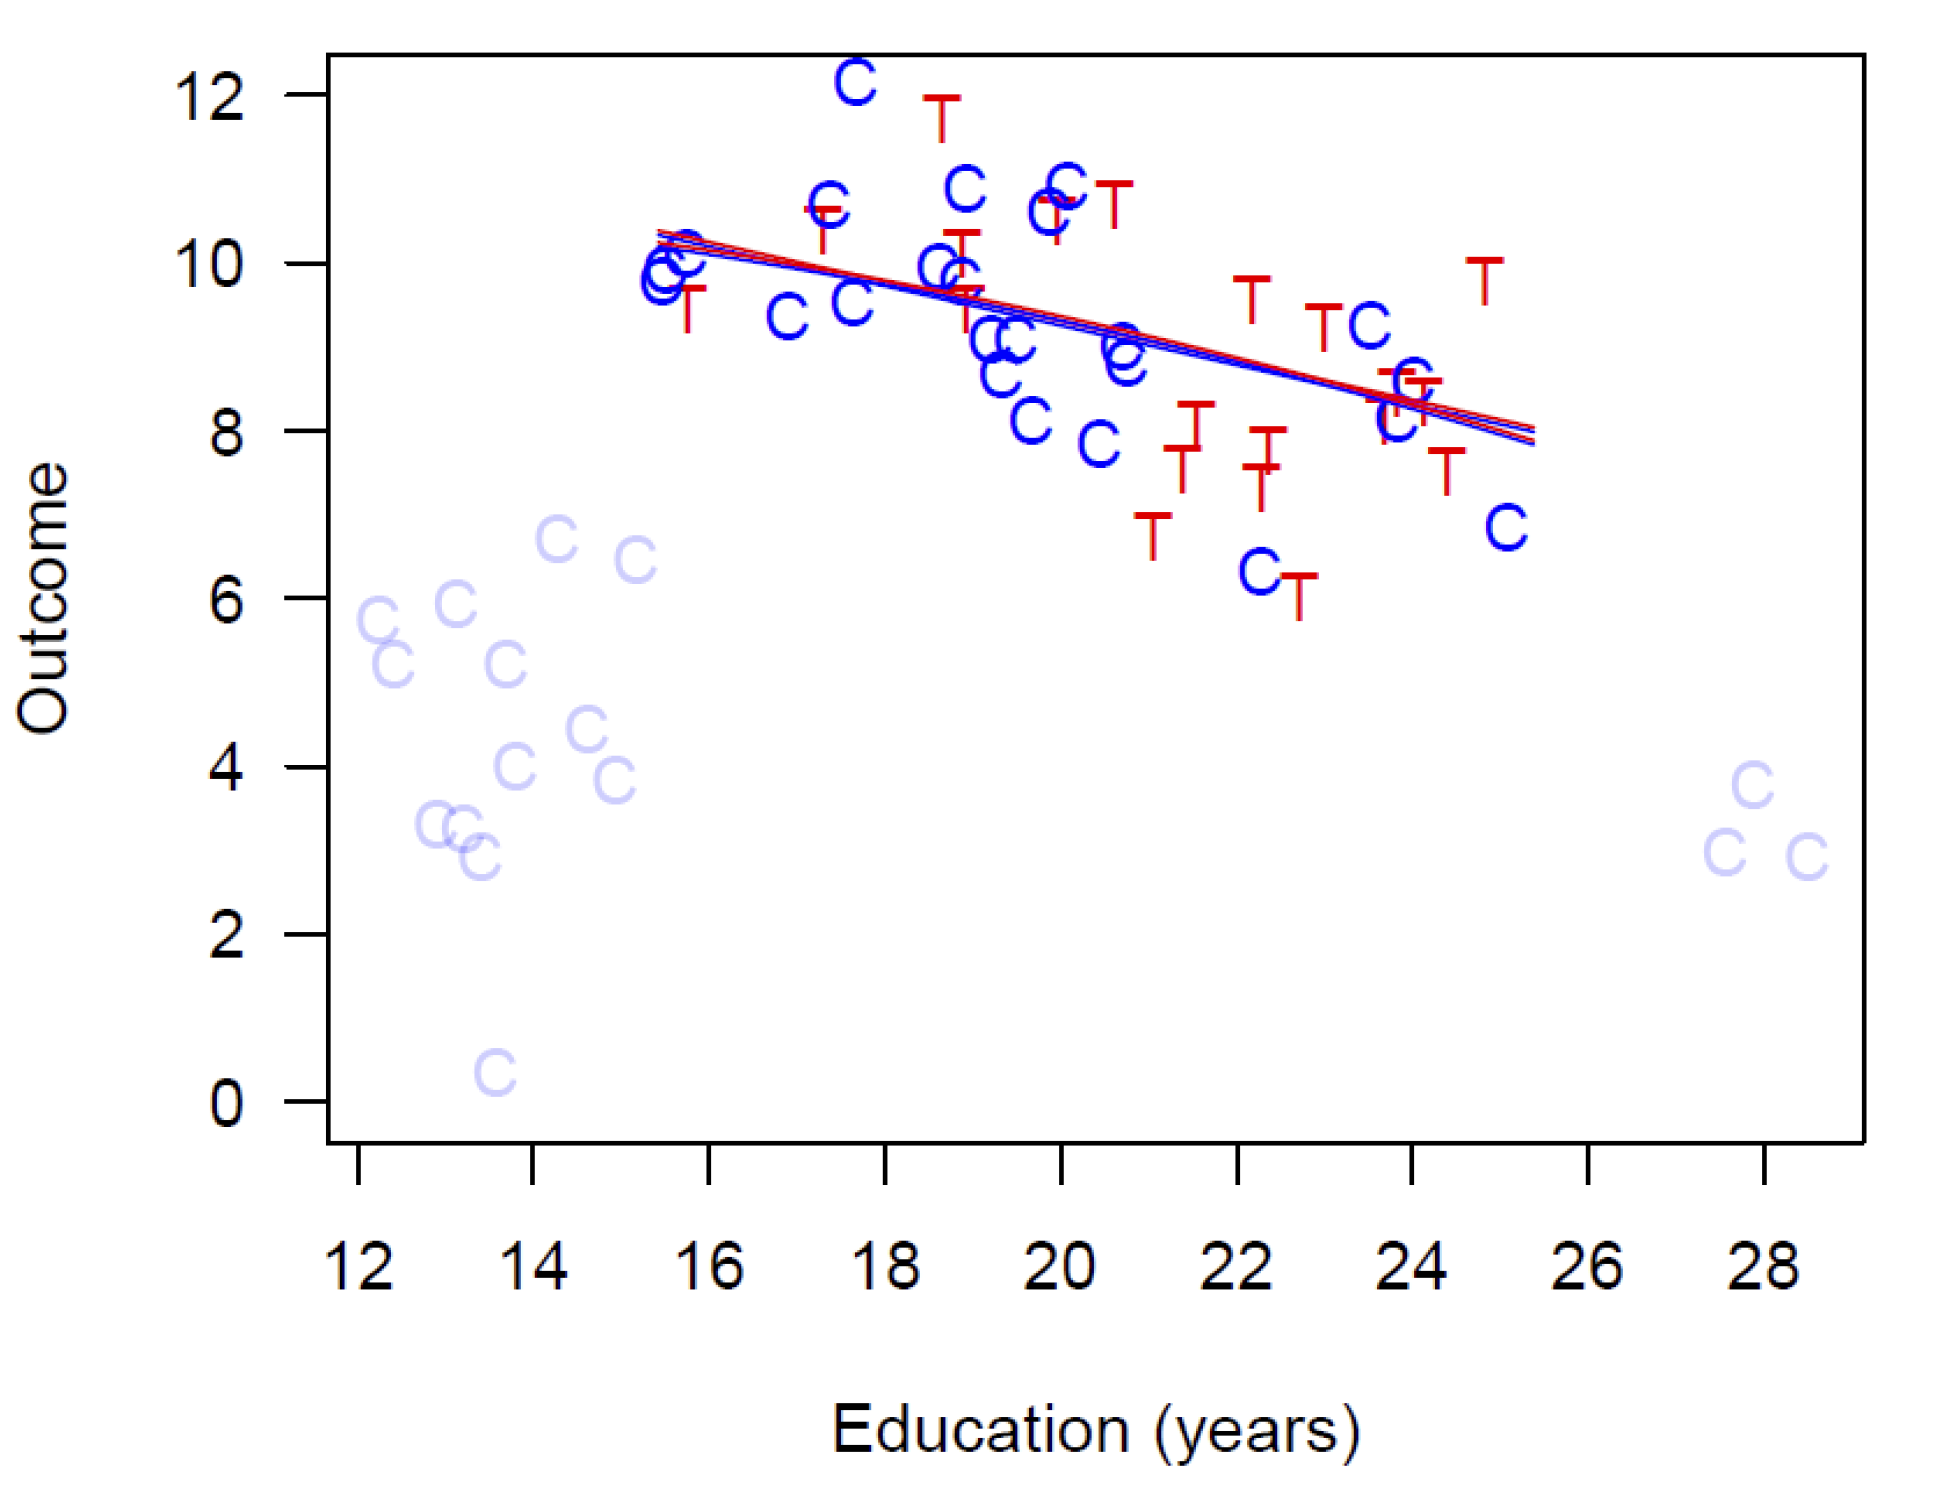
\includegraphics[width=0.7\textwidth]{figure/reg_f6.png}
		\end{figure}
		\begin{minipage}{0.9\linewidth}
			\fontsize{8}{8pt}\selectfont
			\emph{Source:} Ben Elsner's slides
		\end{minipage}
	\end{center}
\end{frame}


\begin{frame}{Regression and Matching}{A Graphical Example}
	\begin{itemize}
		
			\item Among these units within common support region, there is no difference in outcomes between treatment and control groups
	\end{itemize}
\end{frame}



\begin{frame}{Regression and Matching}{Summary}
	\begin{itemize}
		\item When covariate distributions do not overlap, regression must \textbf{extrapolate} into regions where one group is not observed
		\vspace{0.3cm}
		\begin{itemize}
			\item The estimated treatment effect relies entirely on the assumed functional form in those regions
			\vspace{0.2cm}
			\item Results can be sensitive to model misspecification
		\end{itemize}
		\vspace{0.3cm}
		\item Matching avoids extrapolation by restricting comparisons to the \textbf{common support region}
		\vspace{0.3cm}
		\item \textbf{Trade-off between the two approaches:}
		\vspace{0.2cm}
		\begin{itemize}
			\item Matching: no functional form assumptions, but discards observations outside common support
			\vspace{0.2cm}
			\item Regression: uses all data and is more efficient, but risks bias if the functional form is misspecified
		\end{itemize}
	\end{itemize}
\end{frame}


\begin{frame}{Identification Results for Regression}
	\begin{itemize}
		\item We estimate the following regression:	
		\begin{equation*}
			\mathrm{Y}_i = \delta + \alpha D_i + X_{i}\beta + \epsilon_{i}
		\end{equation*}	
		\item The estimated coefficient of treatment $D$ is the following:
		\begin{equation*}
			\alpha = \underbrace{\mathrm{E}[\mathrm{Y}_{i}|X_{i},D_{i}=1] - \mathrm{E}[\mathrm{Y}_{i}|X_{i},D_{i}=0]}_{\text{ODO at given $X_{i}$}} 
		\end{equation*}
		\vspace{0.1cm}
		\item Based on CIA, including all relevant covariates $X_{i}$ into regression can help us eliminate selection bias
		\vspace{0.1cm}
		\item Note: the linear functional form assumption implies $\alpha$ is \textbf{constant} across all values of $X$
	\end{itemize}
\end{frame}

\begin{frame}{Identification Results for Regression}
	\begin{equation*}
	\begin{aligned}
	\alpha =& \underbrace{\mathrm{E}[\mathrm{Y}_{i}|X_{i},D_{i}=1] - \mathrm{E}[\mathrm{Y}_{i}|X_{i},D_{i}=0]}_{\text{ODO at given $X_{i}$}} \\
	&= \underbrace{\mathrm{E}[\mathrm{Y}^{1}_{i}-\mathrm{Y}^{0}_{i}|X_{i},D_i=1]}_{\text{CATT}} 
	+\underbrace{\mathrm{E}[\mathrm{Y}^{0}_{i}|X_{i},D_i=1]-\mathrm{E}[\mathrm{Y}^{0}_{i}|X_{i},D_i=0]}_{\text{Selection Bias}} \\
	&= \underbrace{\mathrm{E}[\mathrm{Y}^{1}_{i}-\mathrm{Y}^{0}_{i}|X_{i},D_i=1]}_{\text{CATT}} + \underbrace{0}_{\text{Selection Bias = 0 by CIA}}  \\
	&=\underbrace{\mathrm{E}[\mathrm{Y}^{1}_{i}-\mathrm{Y}^{0}_{i}|X_{i},D_i=0]}_{\text{CATU}} 
	=\underbrace{\mathrm{E}[\mathrm{Y}^{1}_{i}-\mathrm{Y}^{0}_{i}|X_{i}]}_{\text{CATE}}
	\end{aligned}
	\end{equation*}
	\vspace{0.2cm}
	%\begin{itemize}
   % \item CATT = CATU = CATE because \textbf{CIA} eliminates selection bias at every value of $X_i$, making the distribution of potential outcomes independent of treatment status
	%\end{itemize}
\end{frame}


\begin{frame}{Identification Results for Regression}
	\begin{itemize}	
		\item With continuous or multi-valued covariates $X_i$, we obtain a CATE for each unique value of $X_i$
		\vspace{0.2cm}
		\item Applying the \textbf{law of iterated expectations (LIE)}, we can aggregate CATE into ATE:
		\vspace{0.2cm}
		\begin{equation*}
			\mathrm{ATE} = \mathrm{E}_{X}\left[\mathrm{E}[\mathrm{Y}^{1}_{i}-\mathrm{Y}^{0}_{i}|X_{i}]\right] = \mathrm{E}[\mathrm{Y}^{1}_{i}-\mathrm{Y}^{0}_{i}]
		\end{equation*}
		\vspace{0.1cm}
		\item Under the baseline regression without interaction terms, CATE $= \alpha$ for all $X_i$, so LIE immediately gives ATE $=$ ATT $=$ ATU $= \alpha$
		% \vspace{0.2cm}
		% \begin{itemize}
		% 	\item This is a consequence of \textbf{excluding interaction terms} $D_i \times X_i$ from the model
		% 	\vspace{0.2cm}
		% 	\item If interaction terms are included, CATE varies with $X_i$ and LIE is needed to aggregate into ATE
		% \end{itemize}
	\end{itemize}
\end{frame}


% \begin{frame}{Identification Results for Regression}
% 	\begin{itemize}	
% 			\item With continuous or multi-valued covariates $X_i$, we obtain a different CATE for each unique value of $X_i$
% 		\vspace{0.2cm}
		
% 		\item In practice, researchers often need a single summary measure of treatment effects
% 		\begin{itemize}
% 			\vspace{0.2cm}
% 			\item This allows for simpler interpretation and communication of results
% 		\end{itemize}
% 		\vspace{0.2cm}
% 		\item Again, applying the law of iterated expectations (LIE), we can identify ATT, ATU, and ATE
% 				\vspace{0.2cm}
% 			\begin{itemize}
% 			\item Take average of CATT, CATU, and CATE over all subgroups (all possible X-values)
% 		\end{itemize}
		
% 	\end{itemize}
% \end{frame}



% \begin{frame}{Regression and Matching}{Summary}
% 	\begin{itemize}
% 		\item Regression may face challenges due to lack of common support
% 		\vspace{0.2cm}
% 		\begin{itemize}
% 			\item When covariate distributions do not overlap between treated and control groups
% 			\vspace{0.2cm}
% 			\item Regression must \textbf{extrapolate} into regions where one group is not observed, relying entirely on the assumed functional form
% 			\vspace{0.2cm}
% 			\item Control units outside the common support influence the slope of the regression line, which in turn affects the extrapolated counterfactual
% 			\vspace{0.2cm}
% 		\end{itemize}
% 	\end{itemize}
% \end{frame}

% \begin{frame}{Regression and Matching}{Summary}
% 	\begin{itemize}
% 		\item Matching avoids this issue by restricting comparisons to the common support region
% 		\vspace{0.2cm}
% 		\begin{itemize}
% 			\item Only units with similar covariate values are compared
% 			\vspace{0.2cm}
% 			\item Ensures comparisons are made between fundamentally comparable units
% 			\vspace{0.2cm}
% 			\item Avoids extrapolation to regions without data support
% 			\vspace{0.2cm}
% 		\end{itemize}
		
% 		\item However, matching may discard useful data outside the common support region
% 		\vspace{0.2cm}
% 		\begin{itemize}
% 			\item Regression can potentially utilize this information, if the model is correctly specified
% 			\vspace{0.2cm}
% 			\item \textbf{Trade-off}: regression gains efficiency by using all data, but risks bias if the functional form is misspecified; matching avoids extrapolation bias at the cost of discarding observations
% 		\end{itemize}
% 	\end{itemize}
% \end{frame}

% \begin{frame}{Identification Results for Regression}
	
% 		\begin{itemize}
% \item We estimate the following regression:	
% 		\begin{equation*}
% 		\begin{aligned}
% 			\mathrm{Y}_i &= \delta + \alpha D_i + X_{i}  \beta + \epsilon_{i}
% 		\end{aligned}
% 	\end{equation*}	
	
	
	
% 	\item The estimated coefficient of treatment $D$ is the following:

% \begin{equation*}
% \alpha(X) = \underbrace{\mathrm{E}[\mathrm{Y}_{i}|X_{i},D_{i}=1] - \mathrm{E}[\mathrm{Y}_{i}|X_{i},D_{i}=0]}_{\text{ODO at given $X_{i}$}} 
% \end{equation*}
% \vspace{0.3cm}
% 	\item Based on CIA, including all relevant covariates $X_{i}$ into regression can help us eliminate selection bias 

	
% 		\end{itemize}
% \end{frame}






% \begin{frame}{Identification Results for Regression}
	
	
% 	\begin{equation*}
% 	\begin{aligned}
% 	\alpha(X) =& \underbrace{\mathrm{E}[\mathrm{Y}_{i}|X_{i},D_{i}=1] - \mathrm{E}[\mathrm{Y}_{i}|X_{i},D_{i}=0]}_{\text{ODO at given $X_{i}$}} \\
% 	%&= \mathrm{E}[\mathrm{Y}^{1}_{i}|X_{i},D_i=1]-{\color{red} \mathrm{E}[\mathrm{Y}^{0}_{i}|X_{i},D_i=1]} 
% 	%\\
% 	%& + {\color{red} \mathrm{E}[\mathrm{Y}^{0}_{i}|X_{i},D_i=1]}-\mathrm{E}[\mathrm{Y}^{0}_{i}|X_{i},D_i=0] \\
% 	%&= \underbrace{\mathrm{E}[\mathrm{Y}^{1}_{i}-\mathrm{Y}^{0}_{i}|X_{i},D_i=1]}_{\text{Causal Effect (CATT)}} + \underbrace{\mathrm{E}[\mathrm{Y}^{0}_{i}|X_{i},D_i=1]-\mathrm{E}[\mathrm{Y}^{0}_{i}|X_{i},D_i=0]}_{\text{Selection Bias}} \\
% 	&= \underbrace{\mathrm{E}[\mathrm{Y}^{1}_{i}-\mathrm{Y}^{0}_{i}|X_{i},D_i=1]}_{\text{CATT}} \\ 
% 	&+\underbrace{\mathrm{E}[\mathrm{Y}^{0}_{i}|X_{i},D_i=1]-\mathrm{E}[\mathrm{Y}^{0}_{i}|X_{i},D_i=0]}_{\text{Selection Bias}} \\
% 	&= \underbrace{\mathrm{E}[\mathrm{Y}^{1}_{i}-\mathrm{Y}^{0}_{i}|X_{i},D_i=1]}_{\text{CATT}} + \underbrace{0}_{\text{Selection Bias}}  \\
% 	&=\underbrace{\mathrm{E}[\mathrm{Y}^{1}_{i}-\mathrm{Y}^{0}_{i}|X_{i},D_i=0]}_{\text{CATU}} \\
% 	&=\underbrace{\mathrm{E}[\mathrm{Y}^{1}_{i}-\mathrm{Y}^{0}_{i}|X_{i}]}_{\text{CATE}}
% 	\end{aligned}
% 	\end{equation*}	
	
	
	
% \end{frame}


%\begin{frame}{Identification Results for Regression}{From Conditional to Unconditional Treatment Effects}
%	\begin{itemize}	
%		\item With continuous or multi-valued covariates $X_i$, we obtain a different CATE for each unique value of $X_i$
%		\vspace{0.2cm}
%		
%		\item In practice, researchers often need a single summary measure of treatment effects
%		\begin{itemize}
%			\vspace{0.2cm}
%			\item This allows for simpler interpretation and communication of results
%		\end{itemize}
%		\vspace{0.2cm}
%		
%		\item By applying the law of iterated expectations (LIE), we can aggregate conditional effects into population-level parameters:
%		\vspace{0.2cm}
%		\begin{itemize}
%			\item $\text{ATE} = \mathrm{E}_X[\mathrm{E}[\mathrm{Y}^{1}_{i}-\mathrm{Y}^{0}_{i}|X_{i}]] = \mathrm{E}_X[\text{CATE}(X_i)]$
%			\vspace{0.1cm}
%			\item $\text{ATT} = \mathrm{E}_{X|D=1}[\mathrm{E}[\mathrm{Y}^{1}_{i}-\mathrm{Y}^{0}_{i}|X_{i},D_i=1]] = \mathrm{E}_{X|D=1}[\text{CATT}(X_i)]$
%			\vspace{0.1cm}
%			\item $\text{ATU} = \mathrm{E}_{X|D=0}[\mathrm{E}[\mathrm{Y}^{1}_{i}-\mathrm{Y}^{0}_{i}|X_{i},D_i=0]] = \mathrm{E}_{X|D=0}[\text{CATU}(X_i)]$
%		\end{itemize}
%		
%	\end{itemize}
%\end{frame}
%








\title[]  
{Estimation}


\author 
{}

%\institute{Institute of Economics, Academia Sinica  \\ Econ, NTU}
%\institute{Institute of Economics, Academia Sinica  \\ IMES/IDAS, NCCU}
\institute{}

%\author 
%{楊子霆 \\ 中研院經濟所}

%\institute 
%{中正大學國際經濟專題研討}




\date
{}


\begin{frame}{}
	\titlepage
\end{frame}



\begin{frame}{Estimation Methods}
	\begin{itemize}
		\item So far, we've discussed \textbf{identification}: under what conditions can regression coefficients be interpreted as causal effects
		\vspace{0.3cm}
		
		\item Now we turn to \textbf{estimation}: how do we obtain numerical values for these causal parameters?
		\vspace{0.3cm}
		
		\item Multiple estimation methods exist:
		\begin{itemize}
			\item Ordinary Least Squares (OLS)
			\item Maximum Likelihood Estimation (MLE)
		\end{itemize}
	\end{itemize}
\end{frame}


\begin{frame}{Review: Ordinary Least Squares Estimation}
	\begin{itemize}
		\item Regression analysis assigns values to model parameters ($\delta$, $\alpha$, and $\beta$) to make predicted values $\hat{\mathrm{Y}}_i$ as close as possible to observed values $\mathrm{Y}_i$ 
		\vspace{0.3cm}
		
		\item OLS estimation accomplishes this by choosing values that \textbf{minimize the sum of squared errors (SSE)}
		\begin{equation*}
			(\hat{\delta},\hat{\alpha},\hat{\beta})= \arg\min_{\delta,\alpha,\beta}\dfrac{1}{N}\sum^N_{i=1}(\mathrm{Y}_i-\delta-\alpha D_i-X_i'\beta)^2
		\end{equation*}
		\vspace{0.3cm}
		
%		\item Under the assumptions of:
%		\begin{itemize}
%			\item Linearity
%			\item No perfect multicollinearity
%			\item Exogeneity: $\mathrm{E}[\epsilon_i|D_i,X_i]=0$
%		\end{itemize}
	%	\vspace{0.2cm}
		
		\item OLS provides consistent estimates of the causal parameters we identified earlier
		
	\end{itemize}
\end{frame}


%
%\begin{frame}{Review: Ordinary Least Squares Estimation}
%
%\begin{itemize}
%\item Regression analysis assigns values to model parameters ($\delta $ and $\alpha$) so as to make $\hat{\mathrm{Y}_i}$ as close as possible to $\mathrm{Y}_i$ 
%\vspace{0.3cm}
%\item Ordinary Least Squares (OLS) estimation accomplish it by choosing values that \textbf{minimize the sum of squared error (SSE)}
%\begin{equation*}
%	(\hat{\delta},\hat{\alpha})= \min_{\delta,\alpha}\dfrac{1}{N}\sum^N_{i=1}(\mathrm{Y}_i-\delta-\alpha D_i)^2
%	\end{equation*}
%\vspace{0.3cm}
%\item The result is the best-fitting line that describes the relationship between $D$ and $Y$ in the sample
%
%
%
%	
%	
%\end{itemize}
%
%\end{frame}




\begin{frame}{Review: Ordinary Least Squares Estimation}{A Graphical Example}
	\begin{center}
		\begin{figure}[p]
			\centering
			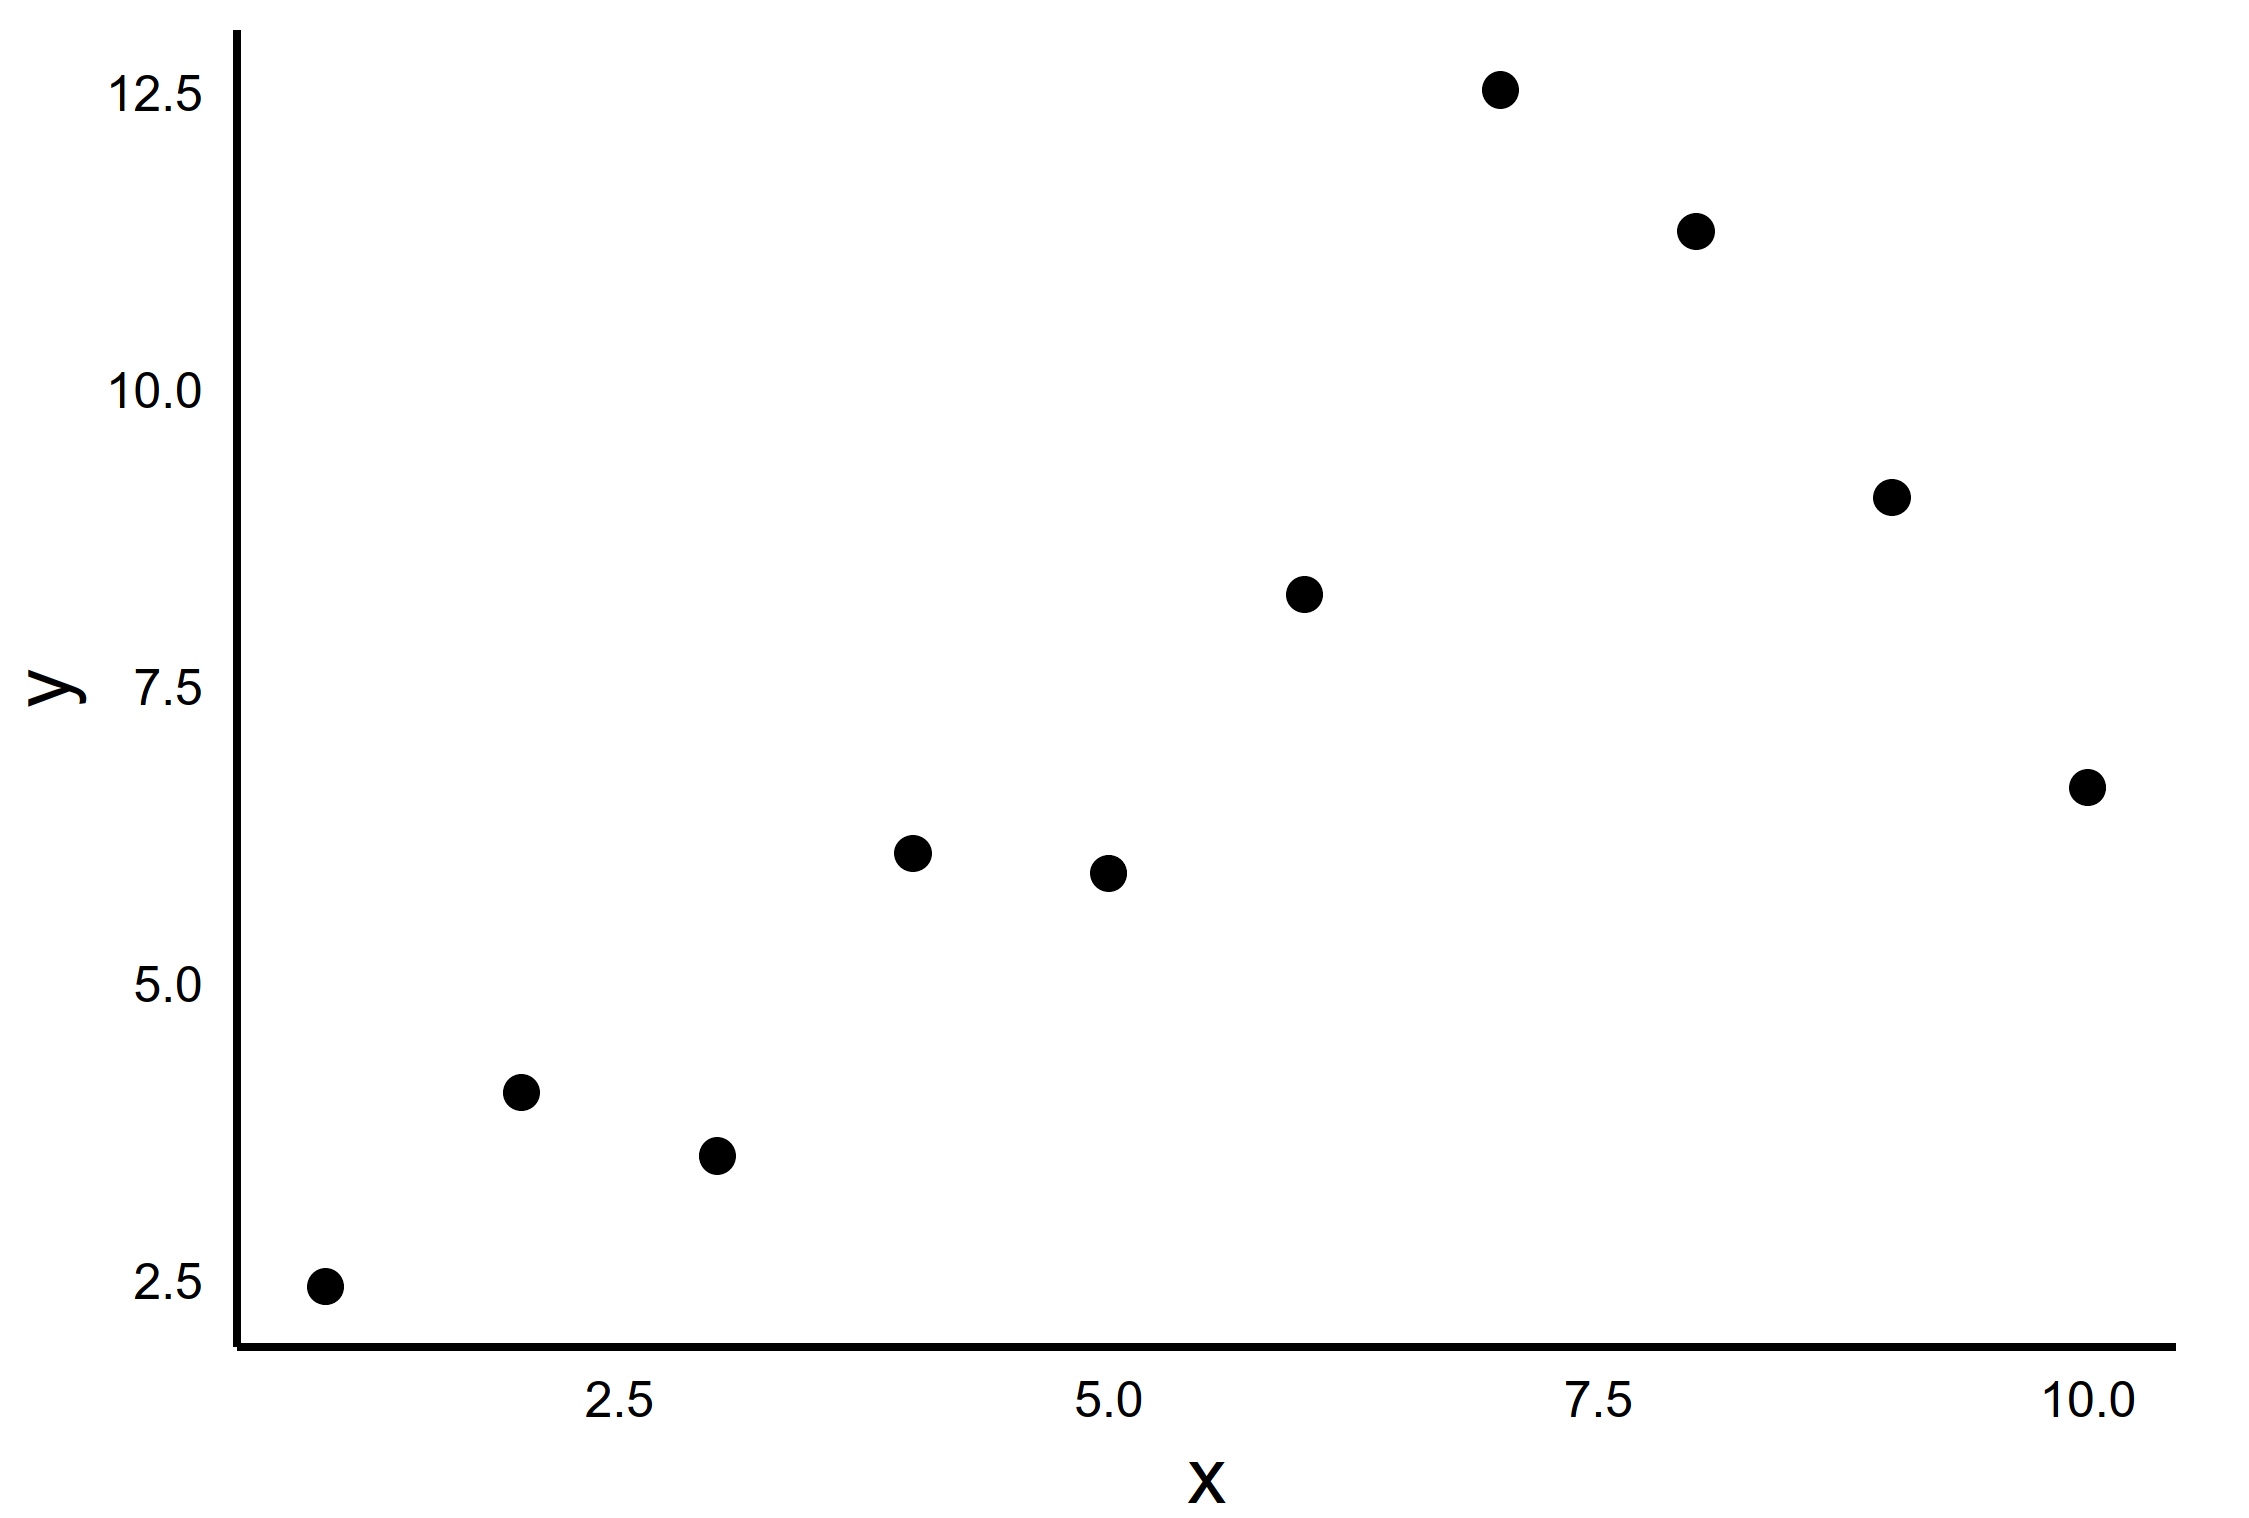
\includegraphics[width=0.7\textwidth]{figure/OLS_f1.png}
		\end{figure}
		\begin{minipage}{0.9\linewidth}
			\fontsize{8}{8pt}\selectfont
			\emph{Source:} Ben Elsner's slides
		\end{minipage}
	\end{center}
\end{frame}




\begin{frame}{Review: Ordinary Least Squares Estimation}{A Graphical Example}
	\begin{center}
		\begin{figure}[p]
			\centering
			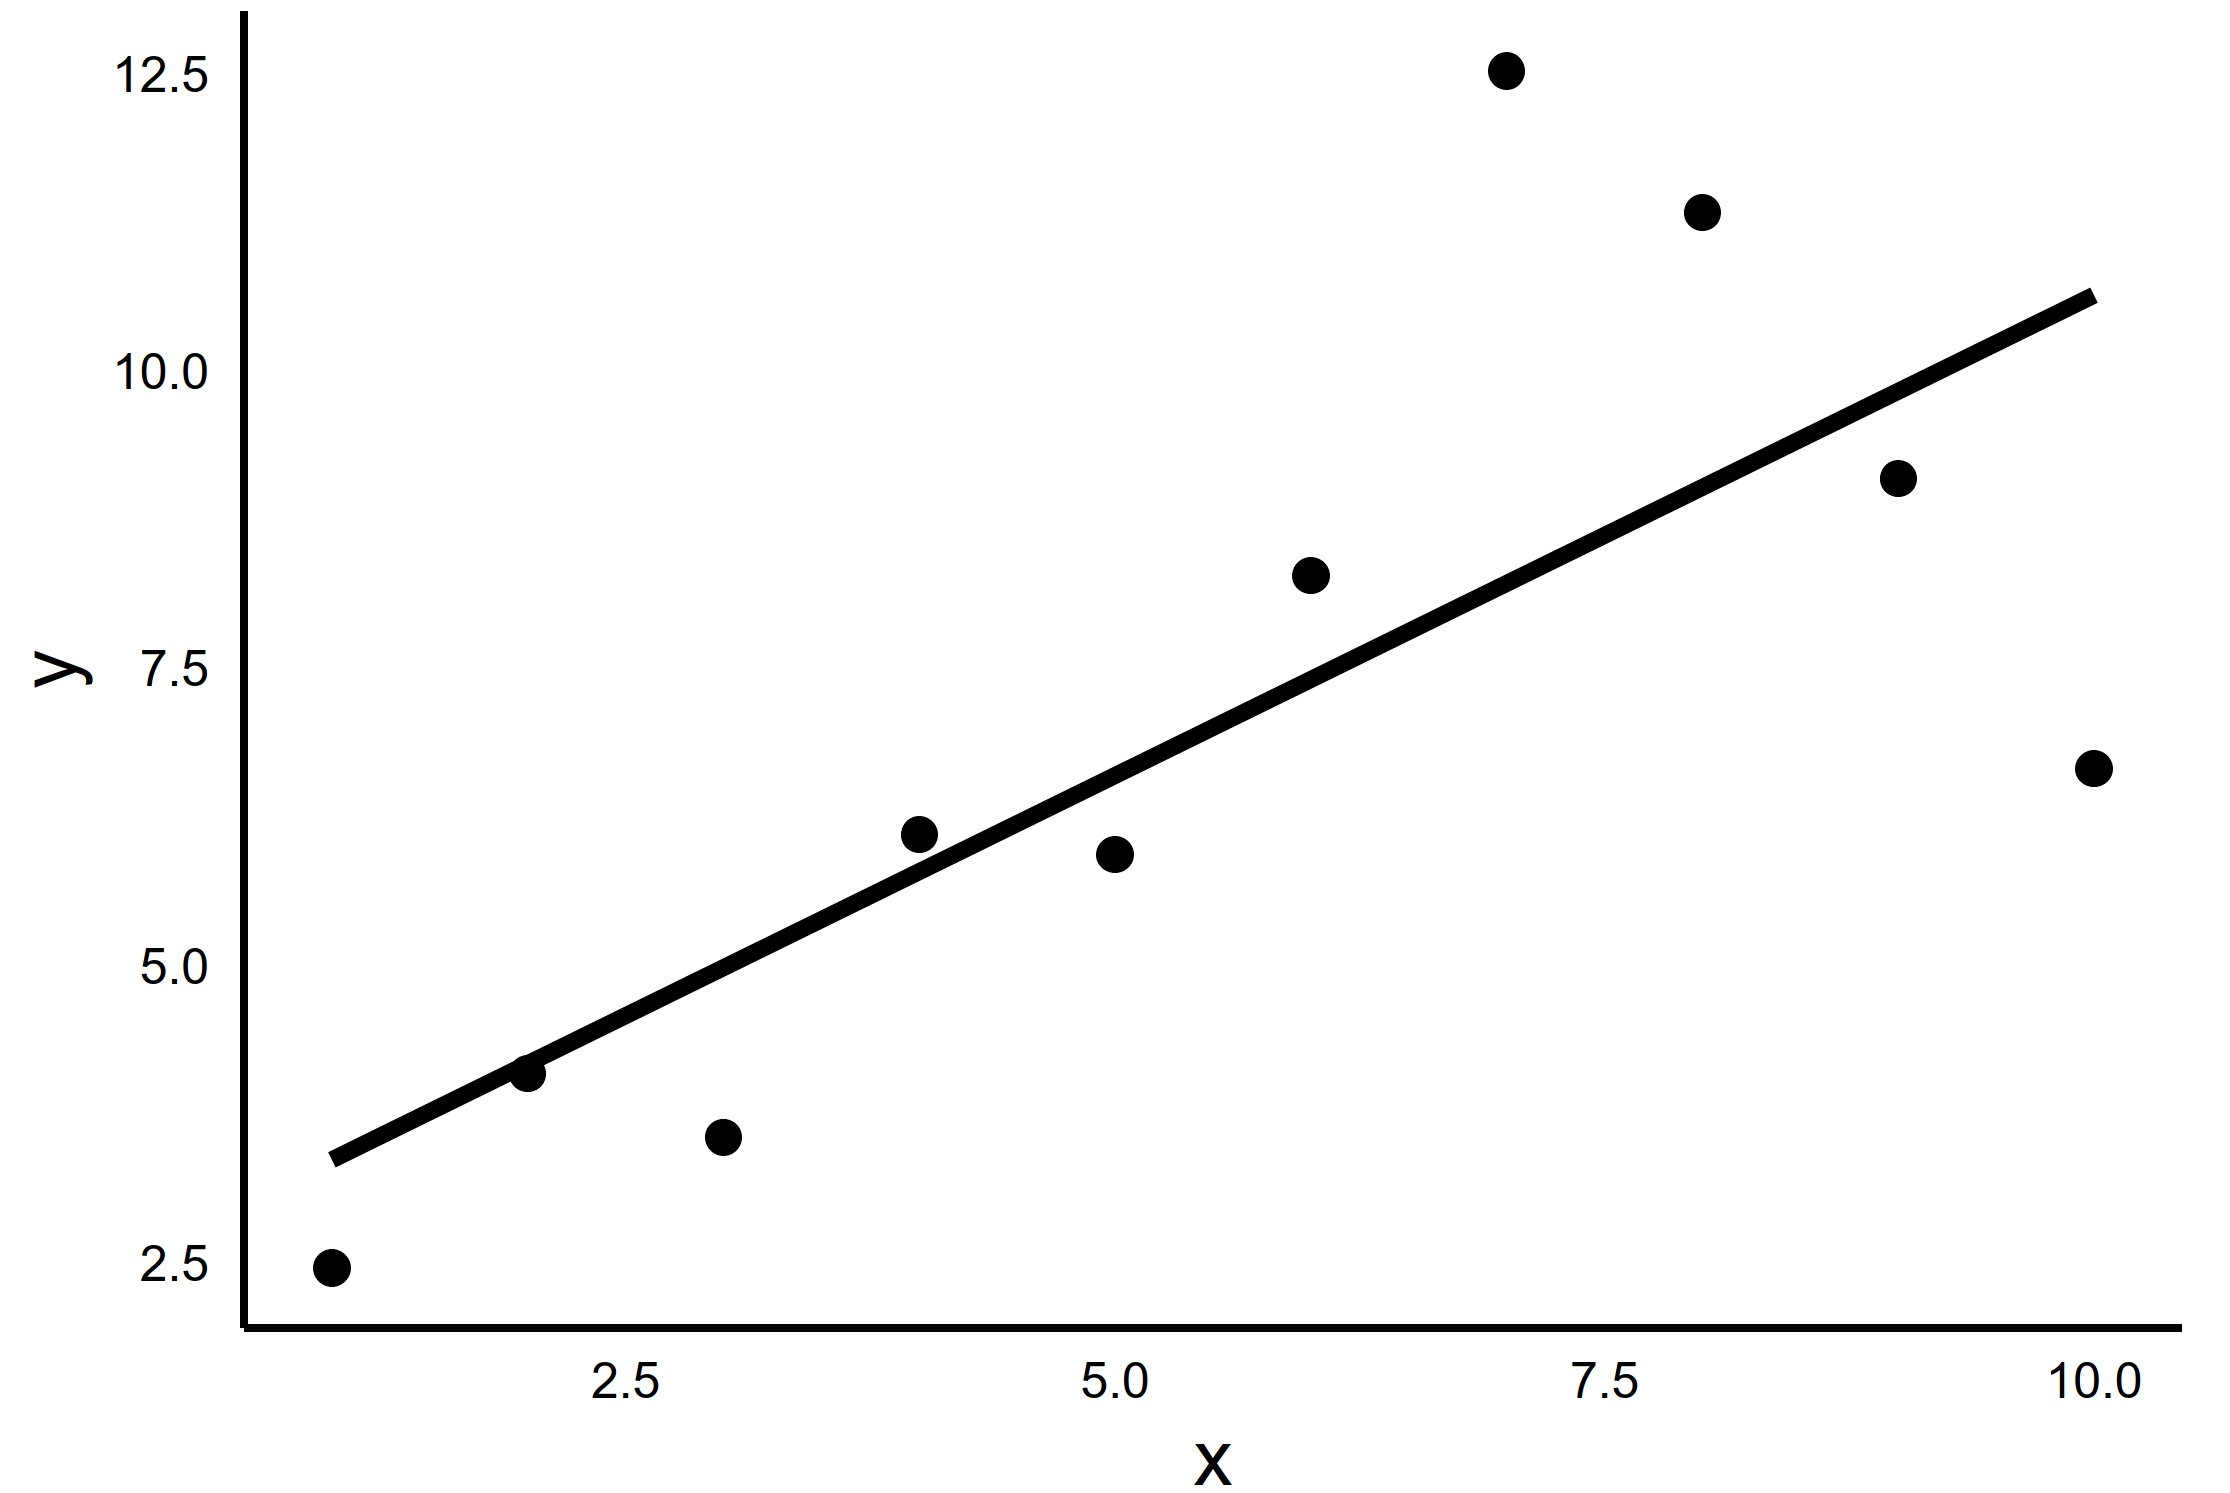
\includegraphics[width=0.7\textwidth]{figure/OLS_f2.png}
		\end{figure}
		\begin{minipage}{0.9\linewidth}
			\fontsize{8}{8pt}\selectfont
			\emph{Source:} Ben Elsner's slides
		\end{minipage}
	\end{center}
\end{frame}




\begin{frame}{Review: Ordinary Least Squares Estimation}{A Graphical Example}
	\begin{center}
		\begin{figure}[p]
			\centering
			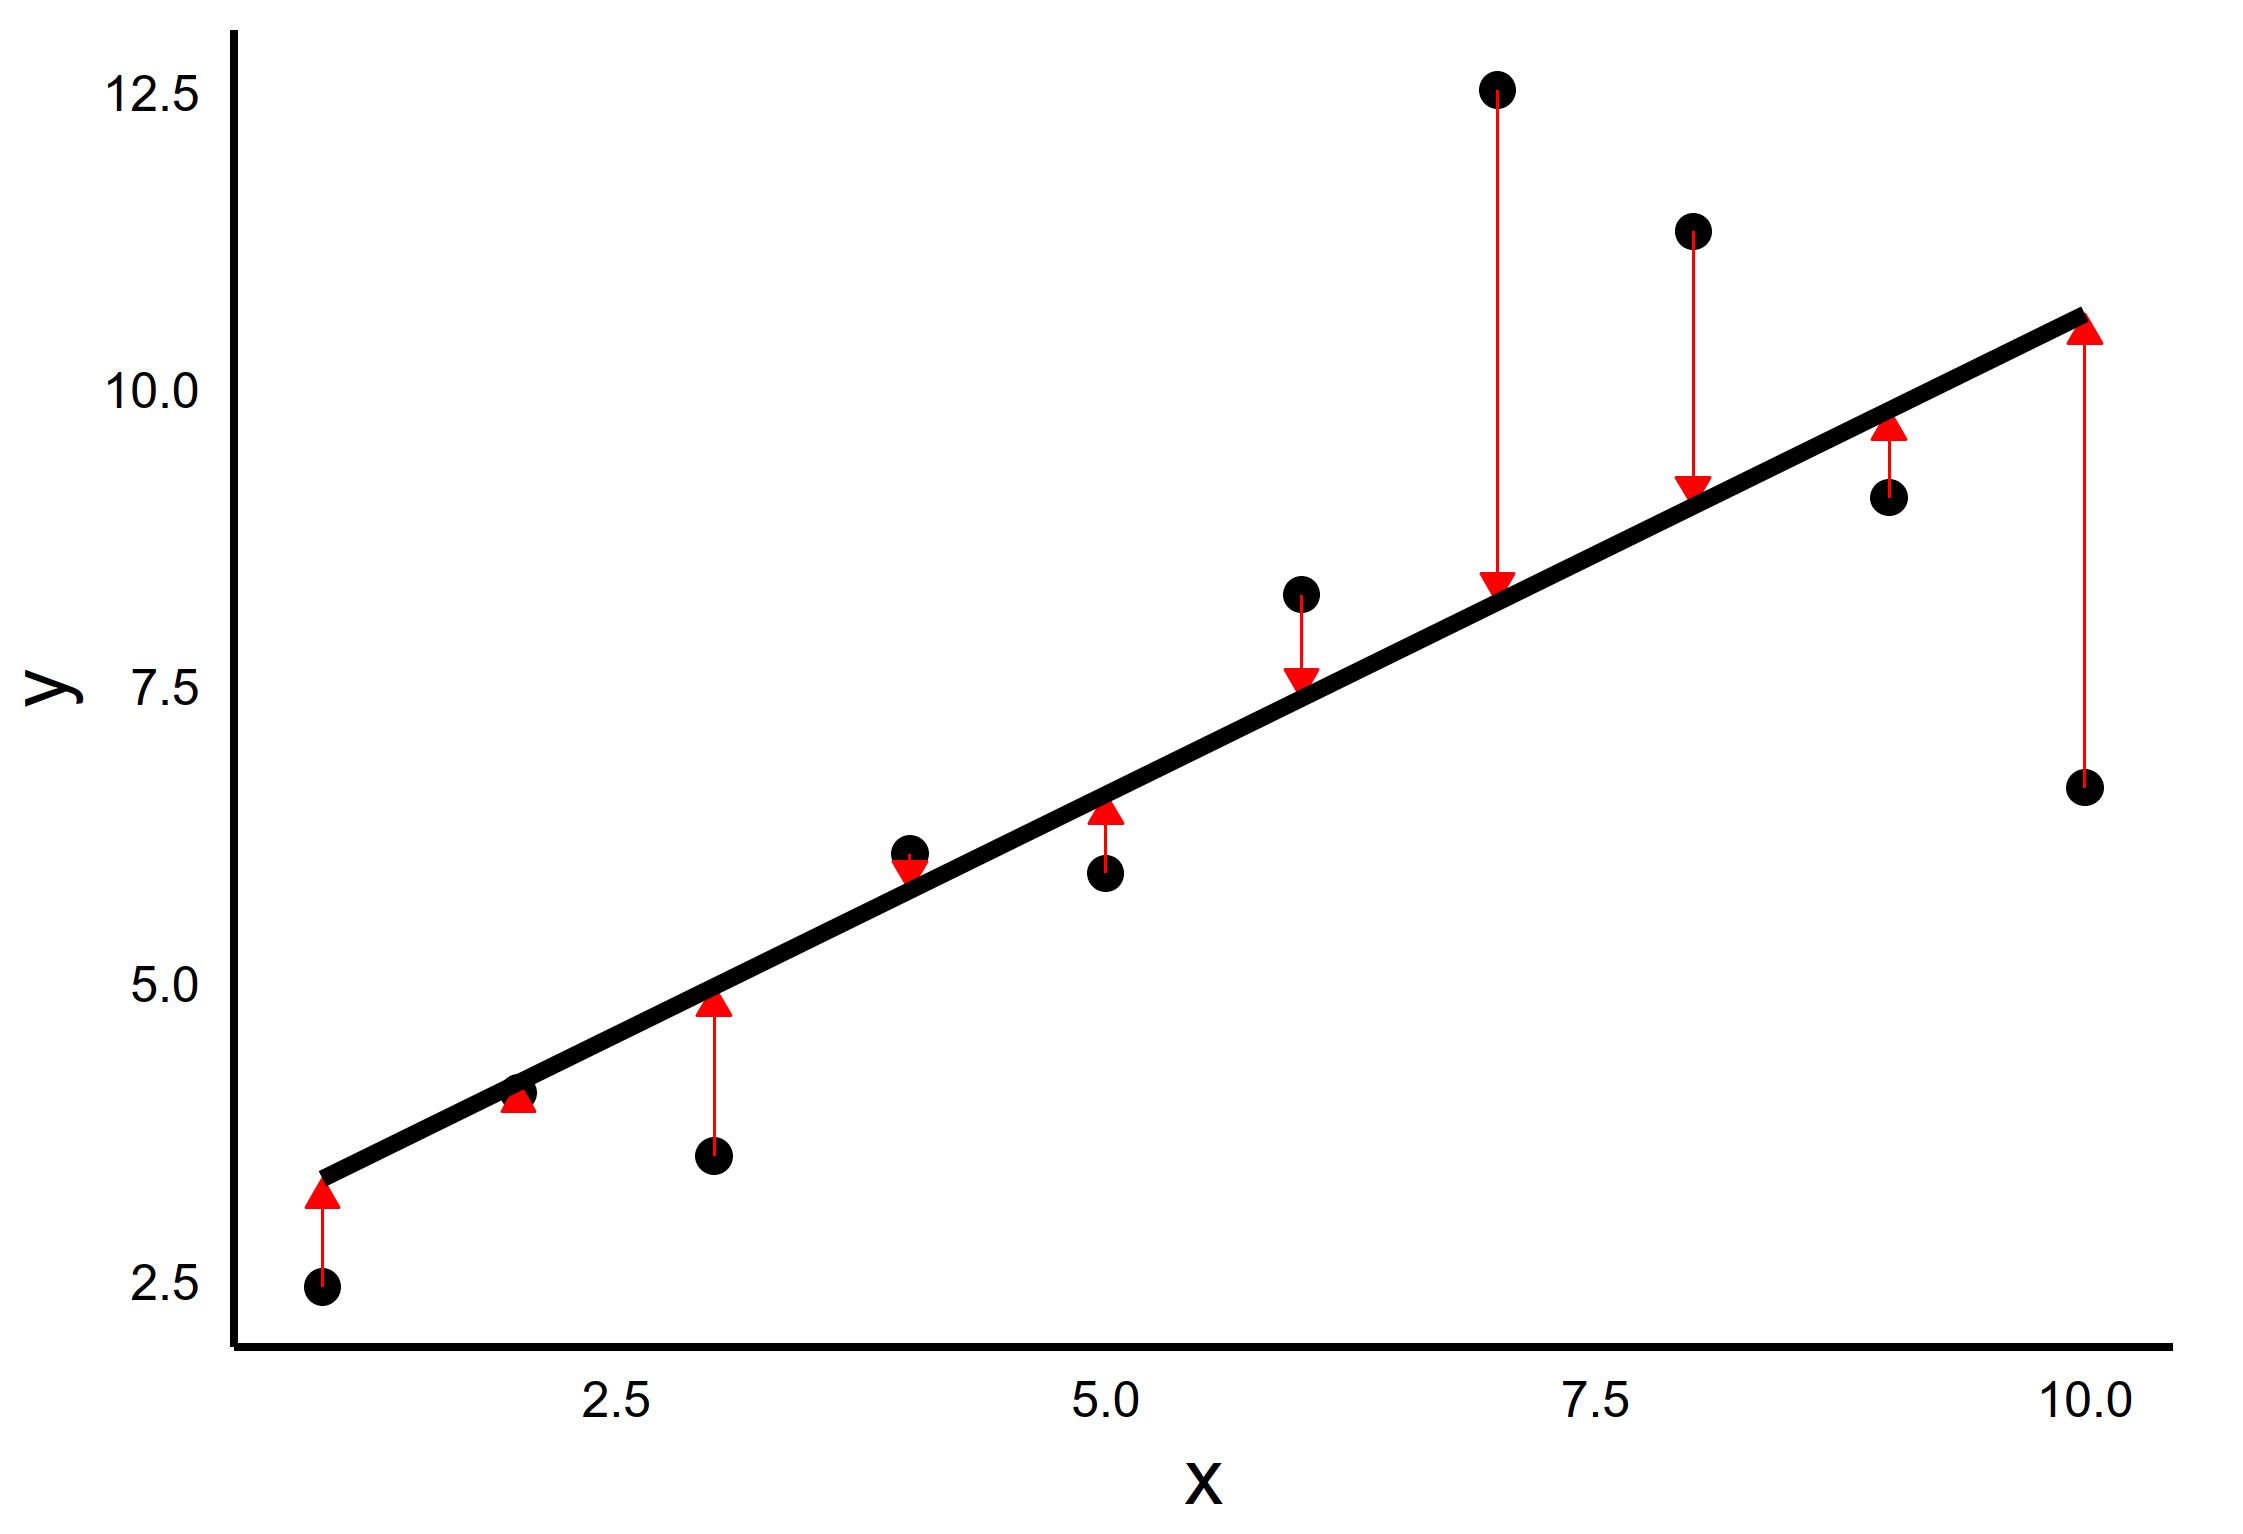
\includegraphics[width=0.7\textwidth]{figure/OLS_f3.png}
		\end{figure}
		\begin{minipage}{0.9\linewidth}
			\fontsize{8}{8pt}\selectfont
			\emph{Source:} Ben Elsner's slides
		\end{minipage}
	\end{center}
\end{frame}



\begin{frame}{Review: Ordinary Least Squares Estimation}{A Graphical Example}
	\begin{center}
		\begin{figure}[p]
			\centering
			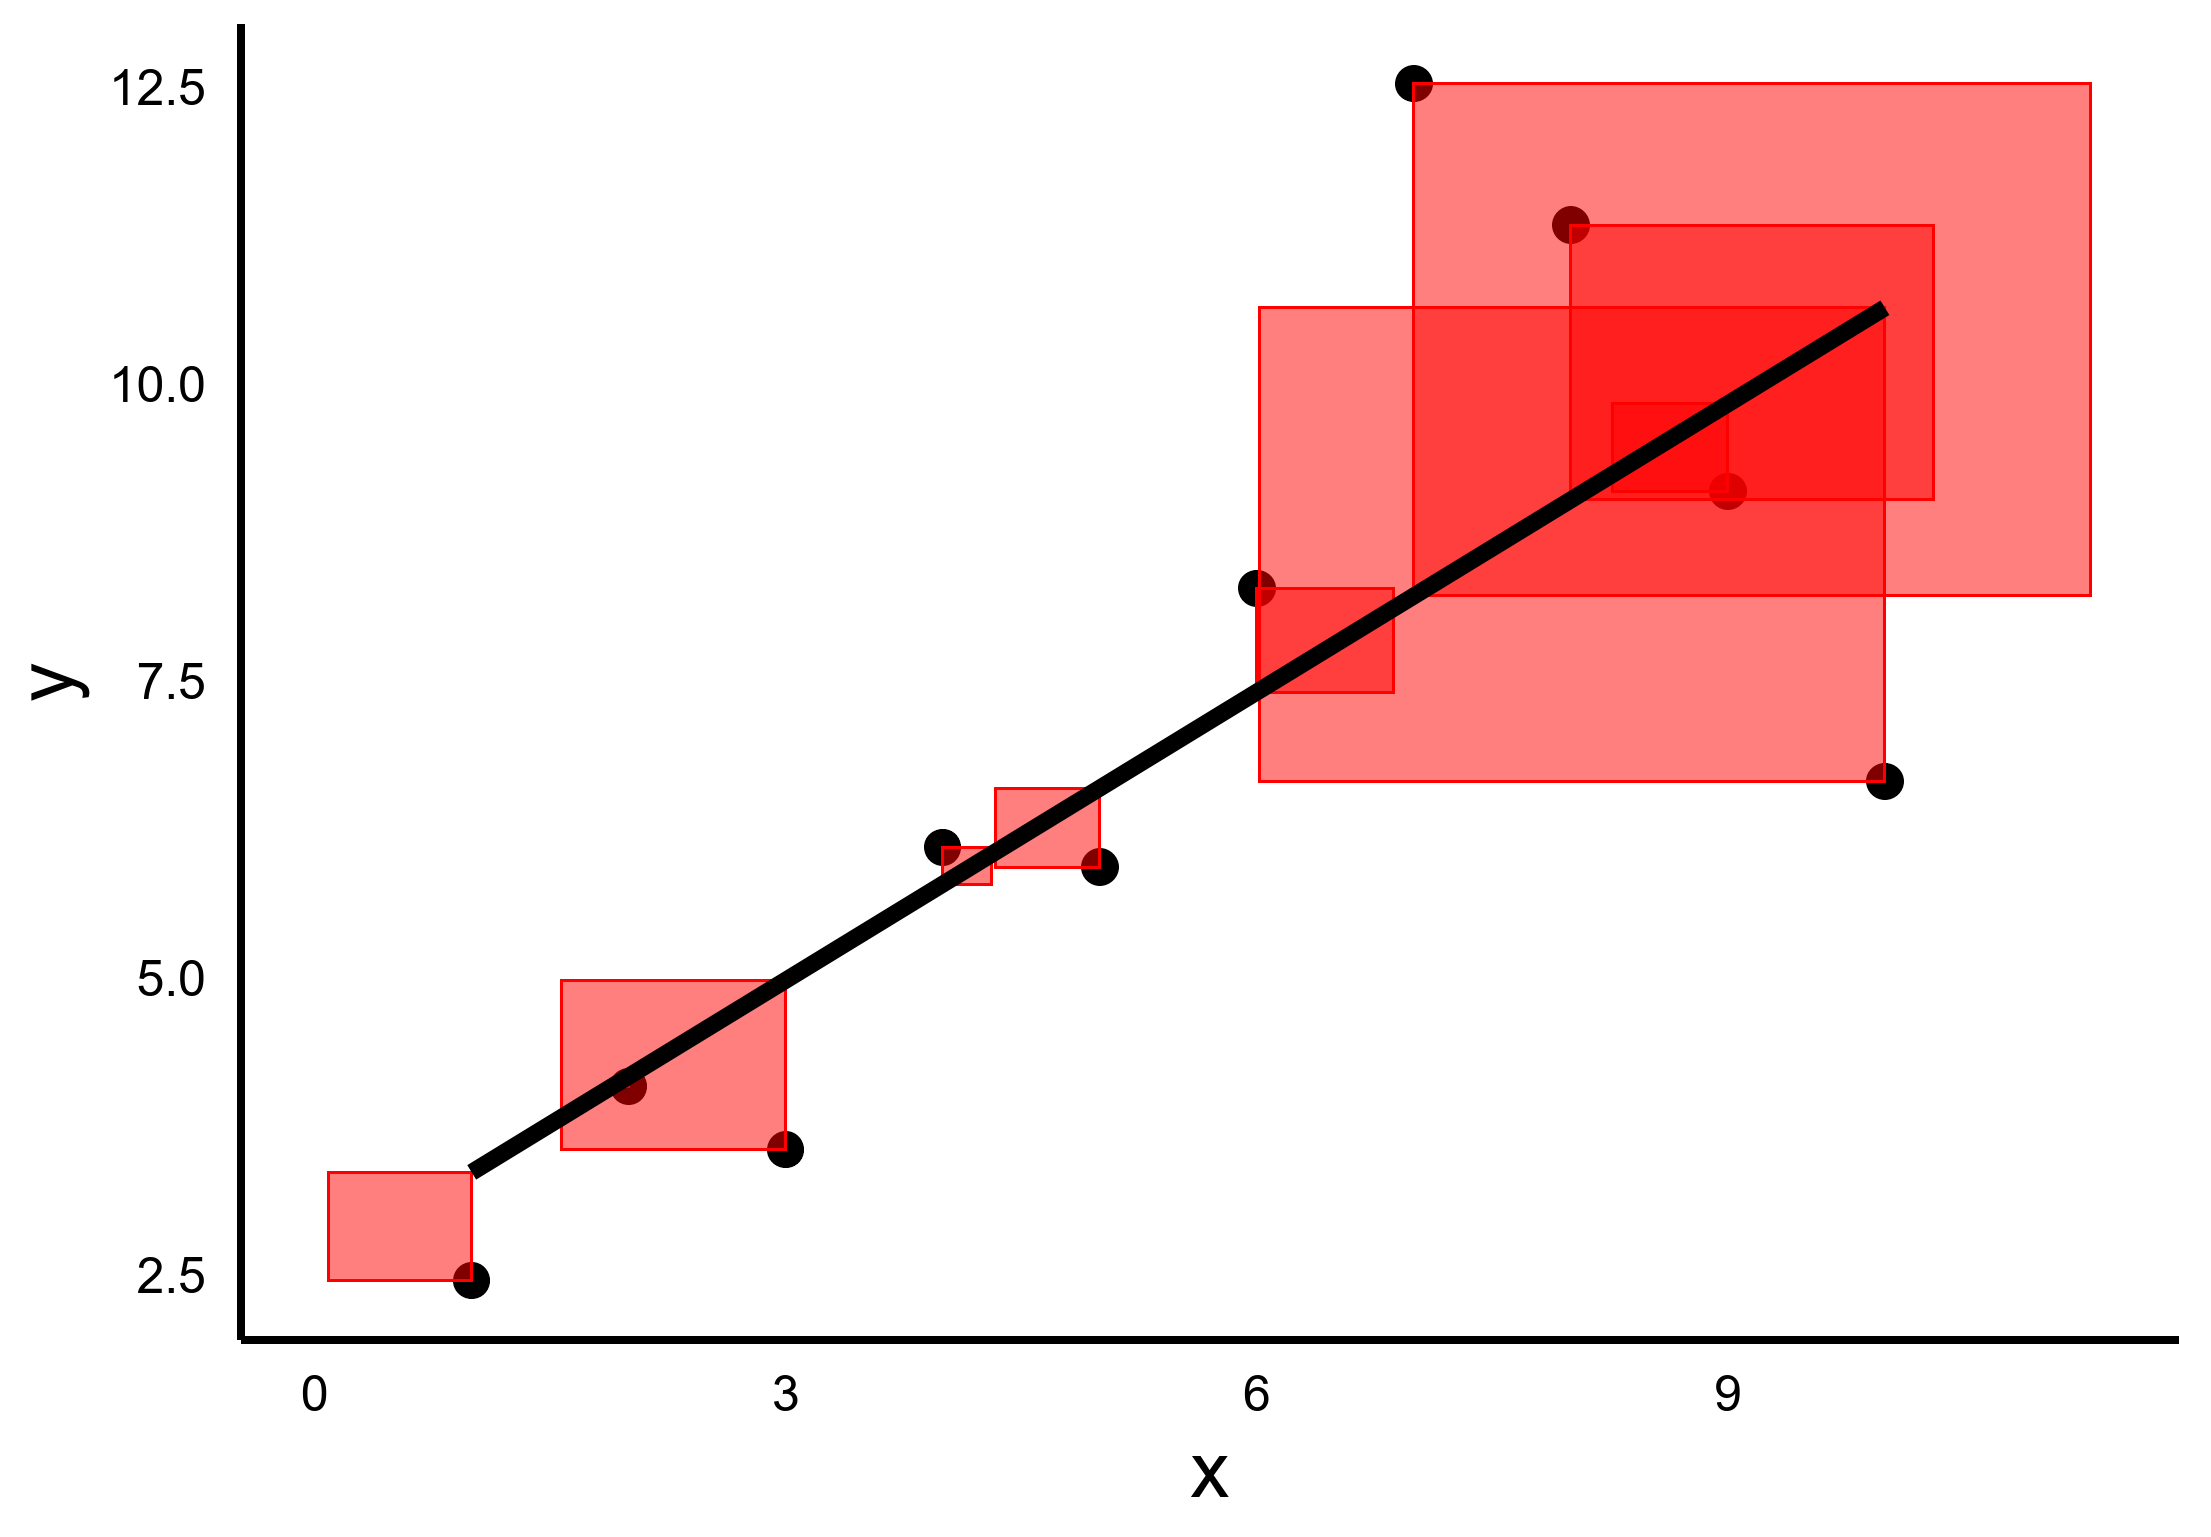
\includegraphics[width=0.7\textwidth]{figure/OLS_f4.png}
		\end{figure}
		\begin{minipage}{0.9\linewidth}
			\fontsize{8}{8pt}\selectfont
			\emph{Source:} Ben Elsner's slides
		\end{minipage}
	\end{center}
\end{frame}



\begin{frame}{Review: Ordinary Least Squares Estimation}{A Graphical Example}
	\begin{center}
		\begin{figure}[p]
			\centering
			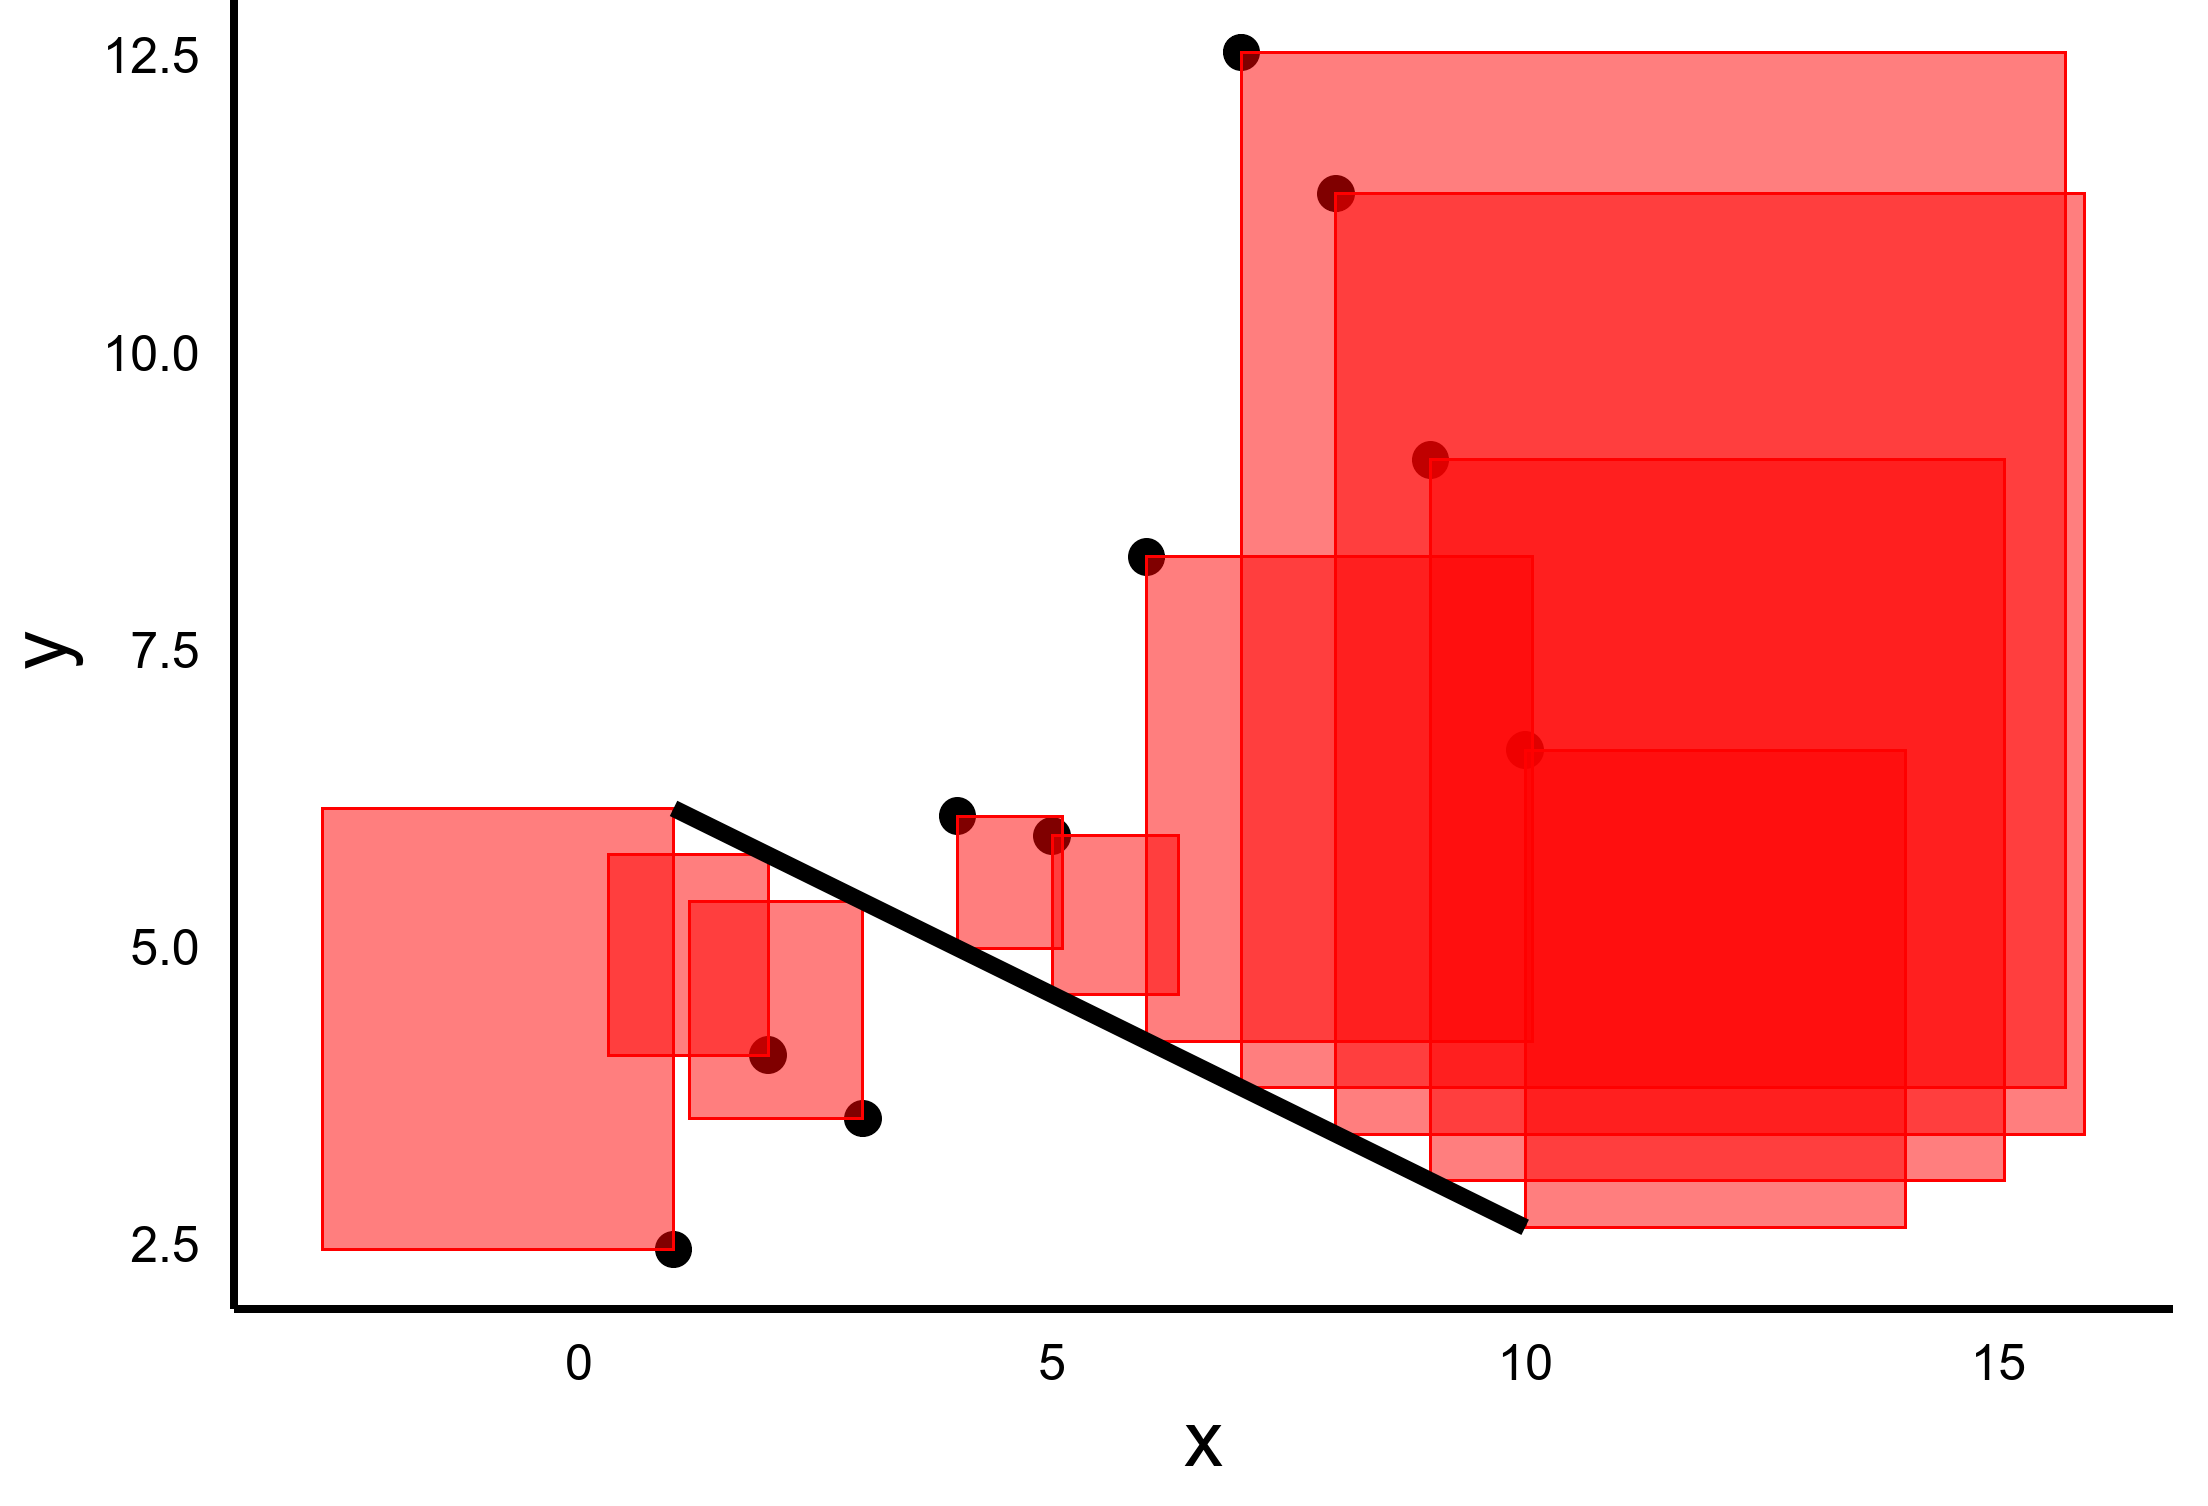
\includegraphics[width=0.7\textwidth]{figure/OLS_f5.png}
		\end{figure}
		\begin{minipage}{0.9\linewidth}
			\fontsize{8}{8pt}\selectfont
			\emph{Source:} Ben Elsner's slides
		\end{minipage}
	\end{center}
\end{frame}




\begin{frame}{Review: Omitted Variable Bias}
	
	\begin{itemize}
		%\item Note that the assignment of treatment in non-experimental data is not random 
		%\vspace{0.3cm}
		%\begin{itemize}
		%\item The treatment and control group may be very different in many characteristics 
		%\vspace{0.3cm}
		%\item These characteristics might be correlated with treatment and affect the outcome variable
		%\vspace{0.3cm}
		%\end{itemize}
		%\item If we do not include these variables into regression model, it will cause Omitted Variable Bias (OVB)
		
		\item OLS estimator for treatment effect $\alpha$: 
		
		\begin{equation*}
			\hat{\alpha} = \dfrac{Cov(\mathrm{Y}_{i},D_{i})}{V(D_{i})}
		\end{equation*}	
		
		
		\item Failure to include enough (right) control variables in the regression would result in selection bias
		\vspace{0.3cm}
		\item The \textbf{OLS version} of the \textbf{selection bias} generated by inadequate controls is called \textbf{Omitted Variable Bias (OVB)}
		
		
	\end{itemize}
	
\end{frame}



\begin{frame}{Review: Omitted Variable Bias}

\begin{itemize}
\item Suppose the true model is:

\begin{align*}
	\mathrm{Y}_i &= \delta + \alpha D_i + \beta X_{i} + \epsilon_{i}
	\end{align*}

\vspace{0.3cm}
\item $X_{i}$ is the observed characteristics (e.g. family wealth)
\vspace{0.3cm}
\item But we estimate this model:
\begin{align*}
	\mathrm{Y}_i &= \delta + \alpha D_i + u_i	
	\end{align*}
	
\begin{itemize}	
\item where $u_i = \beta X_{i} + \epsilon_{i}$
\vspace{0.3cm}
\item Assume $\mathrm{E}[\epsilon_{i}|D_i,X_{i}] = 0$
\end{itemize}	
\end{itemize}

\end{frame}







\begin{frame}{Review: Omitted Variable Bias}

\begin{itemize}


\item OVB formula: 
\begin{equation*}
	\begin{aligned}
   \hat{\alpha} &\overset{p}{\rightarrow} \alpha + \dfrac{Cov(u_{i},D_{i})}{V(D_{i})}  \\	
       &= \alpha + \beta \dfrac{Cov(X_{i},D_{i})}{V(D_{i})}
   	\end{aligned}	
	\end{equation*}


\begin{itemize}
\item Covariance between $X_{i}$ and $D_{i}$: $\text{Cov}(X_i, D_i) = \frac{1}{N} \sum^N_{i=1} (X_i - \bar{X})(D_i - \bar{D})$
\vspace{0.3cm}

\item Variance of $D_{i}$: $V(D_i) = \frac{1}{N} \sum^N_{i=1} (D_i - \bar{D})^2$

\vspace{0.3cm}
\end{itemize}

\item The difference between estimated treatment effect $\hat{\alpha}$ and true effect $\alpha$ depends on two components:
\vspace{0.3cm}
\begin{itemize}
\item[1] $\beta$: The effect of omitted variable $X_{i}$ on outcome variable $\mathrm{Y}_{i}$ 
\vspace{0.3cm}
\item[2] $\dfrac{Cov(X_{i},D_{i})}{V(D_{i})}$: The relationship between omitted variable $X_{i}$ and treatment variable $D_{i}$ 


\end{itemize}
	
\end{itemize}

\end{frame}




\begin{frame}{Review: Omitted Variable Bias}
	\begin{figure}
		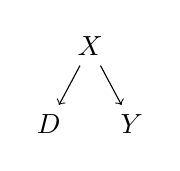
\begin{tikzpicture}[comment/.style={rectangle, text centered}]
		\centering
		\node (u) {$X$};
		\node (D) [below=0.5 of u, xshift=-1.5em] {$D$};
		%\node (Z) [left =1.5em of D] {$Z$};
		\node (Y) [below=0.5 of u, xshift=1.5em] {$Y$};
		
		\draw [->] (u) -- node [auto]{}  (D);
		\draw [->] (u) -- node [auto]{}  (Y);
		%\draw [->] (D) -- node [auto]{}  (Y);
		%\draw [->] (Z) -- node [auto]{}  (D);
		%\draw[<->, >=latex', shorten >=2pt, shorten <=2pt, bend right=30, thick, color=red] 
		%(Z.south) to node[auto, swap] {exclusion restriction}(Y.south);
		%\node  [comment, below = 0.08 of D] (1) {\Large\color{red}$\times$};
		\end{tikzpicture}
	\end{figure}
	
	
	\begin{itemize}
		%\item Treatment $D$ could be associated (correlated) with outcome $Y$ 
		%\vspace{0.2cm}
	

		\item The confounding factor $X$ can result in the co-movement between treatment $D$ and outcome $Y$
				\vspace{0.2cm}
			\item Even if treatment $D$ has no causal effect on outcome $Y$
		
		
		
	\end{itemize}
\end{frame}




\begin{frame}{Review: Omitted Variable Bias}{Example}

\begin{itemize}


\item OVB formula: 
\begin{equation*}
	\begin{aligned}
   \hat{\alpha} &\overset{p}{\rightarrow} \alpha + \dfrac{Cov(u_{i},D_{i})}{V(D_{i})}  \\	
       &= \alpha + \beta \dfrac{Cov(X_{i},D_{i})}{V(D_{i})}
   	\end{aligned}	
	\end{equation*}
\item The difference between estimated effect of attending graduate school $\hat{\alpha}$ and true effect of attending graduate school $\alpha$ depends on two components:
\vspace{0.3cm}
\begin{itemize}
\item[1] $\beta$: The effect of family wealth (omitted) $X_{i}$ on earnings $\mathrm{Y}_{i}$ 
\vspace{0.3cm}
\item[2] $\dfrac{Cov(X_{i},D_{i})}{V(D_{i})}$: The relationship between family wealth $X_{i}$ and attending graduate school $D_{i}$ 


\end{itemize}
	
\end{itemize}

\end{frame}




\begin{frame}{Review: Omitted Variable Bias}{}
	\begin{itemize}
		\item In RCT or other qusi-experimental methods, we can eliminate OVB since treatment assignment $D_{i}$ is unrelated to other confounding factors $X_{i}$ 
		\vspace{0.3cm}
			\begin{itemize}
	\item	$\dfrac{Cov(X_{i},D_{i})}{V(D_{i})}=0$
	\end{itemize}
		
		\vspace{0.3cm}
		\item In the regression, we can eliminate OVB by including all relevant confounding factors $X_{i}$ into regression
		\vspace{0.3cm}
		\begin{itemize}
			\item	$\dfrac{Cov(u_{i},D_{i})}{V(D_{i})}=0$
				\vspace{0.3cm}
			\item When we include $X_{i}$ in regression model, $u_i = \epsilon_{i}$ which is unrelated to treatment status $D_{i}$
		\end{itemize}
		
		
	\end{itemize}
\end{frame}










\begin{frame}{Review: Omitted Variable Bias}{}
\begin{itemize}
\item OVB formula is a tool that allows us to consider the impact of controlling for variables we wish we had
\vspace{0.3cm}
\begin{itemize}
\item We cannot use data to check the consequences of omitted variables that we do not observe
\vspace{0.3cm}
\end{itemize}
\item But we can use the OVB formula to make a educated guess as to the likely consequences of their omission
\begin{equation*}
	\begin{aligned}
   \hat{\alpha} &\overset{p}{\rightarrow}  \alpha + \beta \dfrac{Cov(X_{i},D_{i})}{V(D_{i})}
   	\end{aligned}	
	\end{equation*}
		
\end{itemize}
\end{frame}



       \begin{frame}{Review: Frisch-Waugh-Lovell Theorem}{Main Idea}
       	\begin{itemize}
       		\item Consider the population model:
       		\begin{equation*}
       			Y_i = \delta + \alpha D_i + \beta X_i + \epsilon_i
       		\end{equation*}
       		
       		\item The Frisch-Waugh-Lovell (FWL) Theorem states that the following OLS estimators for $\alpha$ are equivalent:
       		\vspace{0.2cm}
       		\begin{enumerate}
       			\item Direct method: Regressing $Y_i$ on $D_i$ and $X_i$ simultaneously
       			       		\vspace{0.2cm}
       			\item Partitioned method:
       			       		\vspace{0.2cm}
       			\begin{itemize}
       				\item Step 1: Regress $D_i$ on $X_i$, obtain residuals $\tilde{D}_i$
       				       		\vspace{0.2cm}
       				\item Step 2: Regress $Y_i$ on $\tilde{D}_i$
       				       		\vspace{0.2cm}
       			\end{itemize}
       		\end{enumerate}
       		
       		\item The theorem also holds for multiple control variables 
       	\end{itemize}
       \end{frame}
       
    \begin{frame}{Review: Frisch-Waugh-Lovell Theorem}{Key Insights}
       	\begin{itemize}
       		\item Key insights from the partitioned method:
       		       		\vspace{0.2cm}
       		\begin{itemize}
       			\item $\tilde{D}_i$ represents the part of $D_i$ uncorrelated with $X_i$
       			       		\vspace{0.2cm}
       			\item Regressing $Y_i$ on $\tilde{D}_i$ isolates the effect of $D_i$ on $Y_i$, controlling for $X_i$
       		\end{itemize}
       		
       	
       	\end{itemize}
       \end{frame}



%\begin{frame}{Anatomy of Regression and Omitted Variable Bias}{The Frisch-Waugh-Lovell Theorem}
%	\begin{itemize}
%	
%			\item Multivariate regression does two steps simultaneously:
%			\vspace{0.2cm}
%			\begin{enumerate}
%				\item Purges the correlation between $D$ and $X$ from $D$; the residuals $\tilde{D}$ are "what's left" and uncorrelated with $X$
%				\vspace{0.2cm}
%				\item Estimates the effect of $\tilde{D}$ on $Y$, i.e., after purging the correlation between $D$ and $X$
%				\vspace{0.2cm}
%			\end{enumerate}
%
%		\item Why is this important?
%		\vspace{0.2cm}
%		\begin{itemize}
%			\item If $X$ is a confounder, we can purge its influence by including it in the regression
%			\vspace{0.2cm}
%			\item The same holds for more than one control variable
%		\end{itemize}
%		\end{itemize}
%\end{frame}





\title[]  
{Bad Control Problem}


\author 
{}

%\institute{Institute of Economics, Academia Sinica  \\ Econ, NTU}
%\institute{Institute of Economics, Academia Sinica  \\ IMES/IDAS, NCCU}
\institute{}

%\author 
%{楊子霆 \\ 中研院經濟所}

%\institute 
%{中正大學國際經濟專題研討}




\date
{}


\begin{frame}{}
	\titlepage
\end{frame}









\begin{frame}{Bad Control Problem}
	\begin{itemize} 
		\item Controlling for additional covariates increases the likelihood that regression estimates have a causal interpretation
		\vspace{0.2cm}
		\item \textbf{Bad control problem}: More controls are not always better
		\begin{itemize} 
			\vspace{0.2cm}
			\item Bad controls are \textbf{variables that could themselves be outcomes, which are also affected by treatment}
			\vspace{0.2cm}
		\end{itemize}
		
		\item \textbf{The bad control problem would lead to selection bias}
	\end{itemize}
\end{frame}



\begin{frame}{Bad Control Problem}
	\begin{itemize} 
		\item We should \textbf{NOT include bad controls} into regression or matching process 
				\vspace{0.2cm}
			\begin{itemize} 
		\item Even if including them can change estimated coefficients of treatment effect
		\vspace{0.2cm}
			\end{itemize}
		\item Good controls are variables that is \textbf{pre-determined}
		\vspace{0.2cm}
		\begin{itemize}
			\item \textbf{The value of variables have been determined before getting treatment}	
			\vspace{0.2cm}	
			
			\item Whether the variables are pre-determined or not, depending on timing of treatment
			\vspace{0.2cm}	
			\item \textbf{Examples:} 
			\begin{itemize}
				\vspace{0.2cm}	
				\item The effect of master degree on earnings	
				\vspace{0.2cm}			
				\item \textbf{Pre-determined variables:} Gender, age, birth place, father's wealth, mother's wealth
				\vspace{0.2cm}	
				\item \textbf{Bad control variables:} occupation, employment, working industry			
			\end{itemize}
			
		\end{itemize}
		
	\end{itemize}
\end{frame}





\begin{frame}{Bad Control Problem and Selection Bias}{Example}
	\begin{itemize} 
		\item We are interested in the effect of master degree on earnings.
		\vspace{0.2cm}
		\item People can work in two occupations: 
		\begin{itemize} 
			\vspace{0.2cm}
			\item White collar ($W_{i}=1$) 
			\vspace{0.2cm}
			\item Blue collar ($W_{i}=0$)
			\vspace{0.2cm}
		\end{itemize}
		\item Occupation is highly correlated with both education (treatment) and earnings (outcome) 
		\vspace{0.2cm}
		\begin{itemize} 
			\item Occupation is a potential omitted variable, should we include it into our regression ?
			\vspace{0.2cm}
			\item Should we look at the effect of master degree on earnings for those within an occupation (e.g. white collar) ?
		\end{itemize}
	\end{itemize}
\end{frame}


\begin{frame}{Bad Control Problem and Selection Bias}{Example}
	\begin{itemize} 
		\item Note that having a master degree also increases the chance of getting a high-paying white collar job.
		\vspace{0.2cm}
		\item That is, occupational choices are also affect by treatment (get a master degree): \textbf{Bad Controls}
		\vspace{0.2cm}
		%\begin{itemize} 
		%\item Since college degree affects occupation
		%\vspace{0.2cm}
		%\end{itemize}
		
	\end{itemize}
\end{frame}



\begin{frame}{Bad Control Problem and Selection Bias}{Example}
	\begin{itemize} 
		\item Comparisons of earnings by college degree status within an occupation are no longer apples-to-apples comparison
		\vspace{0.2cm}
		\begin{itemize} 
			\item Those who have master degree and white color jobs
			\vspace{0.2cm}
			\item Those who do not have master degree but still have white color jobs
			\vspace{0.2cm}
			\item Two groups are different types of people (e.g. different ability)
		\end{itemize}
		\vspace{0.2cm}
		\item Even if master degree completion is randomly assigned
	\end{itemize}
\end{frame}



\begin{frame}{Bad Control Problem and Selection Bias}{Intuition}
	\begin{itemize} 
		\item If our goal was to estimate the causal effect of having a master degree on earnings, it would be a bad idea to control for occupation
		\vspace{0.2cm}
			\begin{itemize} 
		\item The reason is that one of the main ways that education can affect one's earning is through changing occupation
		\vspace{0.2cm}
			\end{itemize}
		\item If our regression controls for occupation, we might shut down this channel and underestimate the effect of having a master degree
		\vspace{0.2cm}
		\begin{itemize} 
			\item The causal effect of having a master degree on earnings given the occupation does not change
		\end{itemize}
		\vspace{0.2cm}
		\item This is related to the concept of mediation effects, where occupation mediates the relationship between education and earnings
		
	\end{itemize}
\end{frame}





\begin{frame}{Good Controls}{Example}
	\begin{figure}
		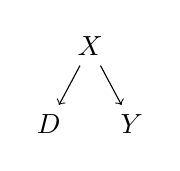
\begin{tikzpicture}[comment/.style={rectangle, text centered}]
			\centering
			\node (u) {$X$};
			\node (D) [below=0.5 of u, xshift=-1.5em] {$D$};
			%\node (Z) [left =1.5em of D] {$Z$};
			\node (Y) [below=0.5 of u, xshift=1.5em] {$Y$};
			
			\draw [->] (u) -- node [auto]{}  (D);
			\draw [->] (u) -- node [auto]{}  (Y);
			%\draw [->] (D) -- node [auto]{}  (Y);
			%\draw [->] (Z) -- node [auto]{}  (D);
			%\draw[<->, >=latex', shorten >=2pt, shorten <=2pt, bend right=30, thick, color=red] 
			%(Z.south) to node[auto, swap] {exclusion restriction}(Y.south);
			%\node  [comment, below = 0.08 of D] (1) {\Large\color{red}$\times$};
		\end{tikzpicture}
	\end{figure}
	
	
	\begin{itemize}
		%\item Treatment $D$ could be associated (correlated) with outcome $Y$ 
		%\vspace{0.2cm}
		
		
		\item  $X$ is the confounding factor and good control variable
		\vspace{0.2cm}
		\item If you want to estimate the (total) effect of treatment $D$, you should control for all confounding factors $X$
		\vspace{0.2cm}
		\item In this case, there is no mediation effect to consider, as $X$ is not on the causal path between $D$ and $Y$
		
		
	\end{itemize}
\end{frame}





\begin{frame}{Bad Controls}{Example}
	\begin{figure}
		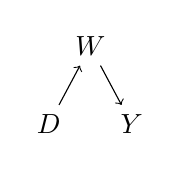
\begin{tikzpicture}[comment/.style={rectangle, text centered}]
			\centering
			\node (u) {$W$};
			\node (D) [below=0.5 of u, xshift=-1.5em] {$D$};
			%\node (Z) [left =1.5em of D] {$Z$};
			\node (Y) [below=0.5 of u, xshift=1.5em] {$Y$};
			
			\draw [<-] (u) -- node [auto]{}  (D);
			\draw [->] (u) -- node [auto]{}  (Y);
			%\draw [->] (D) -- node [auto]{}  (Y);
			%\draw [->] (Z) -- node [auto]{}  (D);
			%\draw[<->, >=latex', shorten >=2pt, shorten <=2pt, bend right=30, thick, color=red] 
			%(Z.south) to node[auto, swap] {exclusion restriction}(Y.south);
			%\node  [comment, below = 0.08 of D] (1) {\Large\color{red}$\times$};
		\end{tikzpicture}
	\end{figure}
	
	
	\begin{itemize}
		%\item Treatment $D$ could be associated (correlated) with outcome $Y$ 
		%\vspace{0.2cm}
		
		
		\item  $W$ is the mediator and bad control variable
		\vspace{0.2cm}
		\item If you want to estimate the (total) effect of treatment $D$, you should NOT control for mediator $W$
		\vspace{0.2cm}
		\item This is because $W$ represents a mediation effect where part of the impact of $D$ on $Y$ flows through $W$
		
		
		
	\end{itemize}
\end{frame}


\begin{frame}{Bad Controls}{Example}
	\begin{figure}
		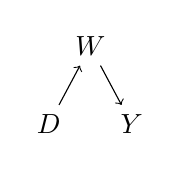
\begin{tikzpicture}[comment/.style={rectangle, text centered}]
			\centering
			\node (u) {$W$};
			\node (D) [below=0.5 of u, xshift=-1.5em] {$D$};
			%\node (Z) [left =1.5em of D] {$Z$};
			\node (Y) [below=0.5 of u, xshift=1.5em] {$Y$};
			
			\draw [<-] (u) -- node [auto]{}  (D);
			\draw [->] (u) -- node [auto]{}  (Y);
			%\draw [->] (D) -- node [auto]{}  (Y);
			%\draw [->] (Z) -- node [auto]{}  (D);
			%\draw[<->, >=latex', shorten >=2pt, shorten <=2pt, bend right=30, thick, color=red] 
			%(Z.south) to node[auto, swap] {exclusion restriction}(Y.south);
			%\node  [comment, below = 0.08 of D] (1) {\Large\color{red}$\times$};
		\end{tikzpicture}
	\end{figure}
	
	
	\begin{itemize}
		%\item Treatment $D$ could be associated (correlated) with outcome $Y$ 
		%\vspace{0.2cm}
		
		
		
		\item However, if you want to estimate the effect of treatment $D$ on outcome $Y$ NOT through the  mediator $W$
		\vspace{0.2cm}
			\begin{itemize}
		\item You can get it by controlling for mediator $W$
		\vspace{0.2cm}
		\item This represents estimating the direct effect rather than the total effect (direct + indirect mediation effect)
		\vspace{0.2cm}
			\end{itemize}
		\item Mediation analysis would decompose the total effect into: direct effect and indirect effect through $W$
		
		
		
		
	\end{itemize}
\end{frame}

\begin{frame}{Mediation Effects}{Decomposition}
	\begin{figure}
		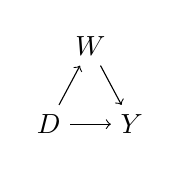
\begin{tikzpicture}[comment/.style={rectangle, text centered}]
			\centering
			\node (u) {$W$};
			\node (D) [below=0.5 of u, xshift=-1.5em] {$D$};
			\node (Y) [below=0.5 of u, xshift=1.5em] {$Y$};
			
			\draw [<-] (u) -- node [auto]{}  (D);
			\draw [->] (u) -- node [auto]{}  (Y);
			\draw [->] (D) -- node [auto]{}  (Y);
		\end{tikzpicture}
	\end{figure}
	
	
	\begin{itemize}
		\item Total Effect = Direct Effect + Indirect Effect
		\vspace{0.2cm}
			\begin{itemize}
		\item Direct Effect: Impact of $D$ on $Y$ not through $W$ (control for $W$)
		\vspace{0.2cm}
		\item Indirect Effect (Mediation Effect): Impact of $D$ on $Y$ through $W$
		\vspace{0.2cm}	
			\end{itemize}
%			\item Typical mediation analysis involves estimating:
%					\vspace{0.2cm}	
%		\begin{itemize}
%			\item Effect of $D$ on mediator $W$
%					\vspace{0.2cm}	
%			\item Effect of mediator $W$ on outcome $Y$ (controlling for $D$)
%					\vspace{0.2cm}	
%			\item Direct effect of $D$ on $Y$ (controlling for $W$)
%		\end{itemize}
	\end{itemize}
\end{frame}




\title[]  
{Statistical Inference}


\author 
{}

%\institute{Institute of Economics, Academia Sinica  \\ Econ, NTU}
%\institute{Institute of Economics, Academia Sinica  \\ IMES/IDAS, NCCU}
\institute{}

%\author 
%{楊子霆 \\ 中研院經濟所}

%\institute 
%{中正大學國際經濟專題研討}




\date
{}


\begin{frame}{}
	\titlepage
\end{frame}





\begin{frame}{Summary of Hypothesis Testing for Regression}
\begin{itemize} 
\item We estimate the following regression and want to test whether there is treatment effect:

\begin{align*}
	Y_i &= \delta + \alpha D_i + X_{i} \beta  + \epsilon_{i}
	\end{align*}
	
\item[1.] Choose a null hypothesis:
	\begin{itemize} 
					\vspace{0.3cm}
	\item We usually test whether there is \textbf{no average effect} of treatment	
	\vspace{0.3cm}
	\item $H_0: \alpha = 0$ 
		\vspace{0.3cm}
	

	\end{itemize}


	
	
	
	

\end{itemize}
\end{frame}







\begin{frame}{Summary of Hypothesis Testing for Regression}
	\begin{itemize} 
	
		
		\item[2.] Choose a test statistic
		\begin{itemize} 
			\vspace{0.3cm}
			\item We use a t-statistic to measure whether our sample estimates support/against this null hypothesis
			
			\vspace{0.3cm}
			\item $t = \dfrac{(\hat{\alpha}-\alpha)}{\hat{\mathrm{SE}}(\hat{\alpha})}$
		\end{itemize}
		
		
		
		
		
	\end{itemize}
\end{frame}




\begin{frame}{Summary of Hypothesis Testing for Regression}
\begin{itemize} 
	
\item[3.] Estimate standard error of the estimator 
	\begin{itemize} 
	\vspace{0.2cm}
	\item $\hat{\mathrm{SE}}(\hat{\alpha})= \sqrt{\dfrac{\sum_{i=1}^{N} \hat{\epsilon}_i^2 \widetilde{D_i}^2}{\left(\sum_{i=1}^{N} \widetilde{D_i}^2\right)^2}}$
	\vspace{0.2cm}
		\begin{itemize} 
   \item \(\hat{\epsilon}_i\) are the residuals from the main regression
   \vspace{0.2cm}
   \item \(\widetilde{D_i}\) are the residuals obtained from regressing \( D_i \) on \( X_i \)
   

\end{itemize}
\vspace{0.2cm}
\item The addition of covariates $X$ has two opposing effects on $\hat{\mathrm{SE}}(\hat{\alpha})$.
	\vspace{0.2cm}
	\begin{itemize} 
\item[1] \(\hat{\epsilon}_i\) might decrease since addition covariates explain some of the variation in $Y_{i}$
	\vspace{0.2cm}
\item[2] \(\widetilde{D_i}\) falls when covariates that predict $D_{i}$ are added to the regressions
	\end{itemize}
\vspace{0.2cm}
\item This is known as \textbf{heteroskedasticity-robust standard errors}
\vspace{0.2cm}
	\begin{itemize} 
\item Provide valid standard errors of estimator $\alpha$ even in the presence of heteroskedasticity (i.e., non-constant variance)
\end{itemize}
\end{itemize}
\end{itemize}
\end{frame}






\begin{frame}{Summary of Hypothesis Testing for Regression}
	\begin{itemize} 
		
		
		
		\item[4.] Evaluate whether the sample estimator is against null hypothesis or not
		\begin{itemize} 
			\vspace{0.3cm}
			\item \textbf{Goal:} Calculate \textbf{p-value}
			\vspace{0.3cm}
			\begin{itemize} 
				\item \textbf{p-value:} Given null hypothesis is true, the probability of obtaining the sample estimates or more extreme ones
				\vspace{0.3cm}

					\item If this probability is high, it means the sample estimate might support for null hypothesis
					\vspace{0.3cm}
					\item If this probability is low, it means the sample estimate might be against null hypothesis		

				
				%a result that is equal to or more extreme than what was actually observed in the sample	
			\end{itemize}
			
			
			
			
			
			
			%against the alternative $H_1: \alpha_{ATE}\neq 0$ at the $5\%$ significance level if $|t|>1.96$
		\end{itemize}	
		
		
		
		
		
		
	\end{itemize}
\end{frame}




\begin{frame}{Summary of Hypothesis Testing for Regression}
	\begin{itemize} 
		
		
		
		\item[4.] Evaluate whether the sample estimator is against null hypothesis or not
		\begin{itemize} 
			\vspace{0.3cm}
			\item In order to calculate this probability (p-value), we need to know the distribution of the t-statistic under the null hypothesis
			\begin{itemize} 
				\vspace{0.3cm}
				\item If sample size is sufficiently large, using \textbf{Central Limit Theorem (CLT)}, t-statistic will have standard normal distribution 
			\end{itemize}
			
			
			
			
			
			
			
			%against the alternative $H_1: \alpha_{ATE}\neq 0$ at the $5\%$ significance level if $|t|>1.96$
		\end{itemize}	
		
		
		
		
		
		
	\end{itemize}
\end{frame}








\begin{frame}{Summary of Hypothesis Testing for Regression}
	\begin{itemize} 
		
		
		
		\item[4.] Evaluate whether the sample estimator is against null hypothesis or not
		\begin{itemize} 
			
			\vspace{0.3cm}
			\item Based on standard normal distribution	and sample estimator, we can get p-value	
			\vspace{0.3cm}
			\item We reject the null hypothesis $H_0: \alpha=0$ when p-value is sufficiently low 	 
			\vspace{0.3cm}
			\begin{itemize} 
				\item We usually select an arbitrarily pre-defined threshold value $\theta$, which is referred to as the \textbf{level of significance}
				\vspace{0.3cm}	
				\item By convention, $\theta$ is commonly set to 0.1 or 0.05
			\end{itemize}	
			\vspace{0.3cm}	
			\item If p-value is smaller than $\theta$, we would say the sample estimate is \textbf{significantly different from the null hypothesis}
			%against the alternative $H_1: \alpha_{ATE}\neq 0$ at the $5\%$ significance level if $|t|>1.96$
		\end{itemize}	
		
		
		
		
		
		
	\end{itemize}
\end{frame}




\begin{frame}{Interpretation of Regression Results}
	\begin{itemize}
		
		\item We are only interested in $\alpha$, the causal effect of treatment $D$ on $Y$
		\vspace{0.2cm} 
		\begin{itemize}
			\item The other coefficients $\beta_1, \beta_2, \ldots, \beta_k$ are NOT of interest
			\vspace{0.2cm} 
			\item We include the covariates $X$ to control for observed confounding factors
			
		\end{itemize}
		\vspace{0.2cm} 
		\item Interpretation of $\alpha$ when controlling $X$
		
		\vspace{0.2cm} 
		\begin{itemize}
			\item Holding all other variables $X$ constant, a one unit increase in $D$ leads to a $\alpha$ unit increase in $Y$
			\vspace{0.2cm} 
		\end{itemize}
		
		
	\end{itemize}
\end{frame}



\begin{frame}{Interpretation of Regression Results}
\begin{itemize} 
\item Suppose the estimated regression is the following:


\begin{align*}
	\hat{\mathrm{Y_{i}}} &= 35000 + 5000 D_{i} + 0.5 X_{i}
	\end{align*}

\item Suppose the estimated standard error is:

\begin{equation*}
	\hat{\mathrm{SE}}(\hat{\alpha})= 1000 
	\end{equation*}
\item So the t-statistic for testing $H_{0}: \alpha=0$:

\begin{equation*}
t = \dfrac{(\hat{\alpha}-\alpha)}{\hat{\mathrm{SE}}(\hat{\alpha})} = \dfrac{5000-0}{1000} = 5
	\end{equation*}

\end{itemize}
\end{frame}



\begin{frame}{Interpretation of Regression Results}
\begin{itemize} 
\item Using t-statistic, we can compute the p-value = $0.00001$, which is much lower than $0.05$ or $0.01$
	\vspace{0.3cm}
	\begin{itemize} 
		
\item Given null hypothesis $H_0: \alpha=0$ is true, our estimate is unlikely to happen (but it happens!!) 		
			\vspace{0.3cm}
\item It suggests our estimate is against the null hypothesis
			\vspace{0.3cm}
\item Thus, we should reject the null hypothesis
\end{itemize}

\end{itemize}



\end{frame}




%\begin{frame}{Interpretation of Regression Results}
%	\begin{itemize} 
%	
%		
%		\item Based on sample estimates and its standard deviation, we can construct a confidence interval for $\alpha$
%		\vspace{0.3cm}
%		\item Note that the t-statistic for 5\% two-sided significance level is 1.96
%		\vspace{0.3cm}
%		\begin{equation*}
%			\hat{\alpha} \pm 1.96 \hat{\mathrm{SE}}(\hat{\alpha})= 5000 \pm 1.96 \times 1000
%		\end{equation*}
%		
%		\begin{itemize} 
%			\item The 95\% confidence interval does not include zero
%			\vspace{0.3cm}
%			\item Null hypothesis $H_{0}: \alpha=0$ is rejected at the 5\% level
%		\end{itemize}
%		
%		
%	\end{itemize}
%\end{frame}









\begin{frame}{Interpretation of Regression Results}{When $Y$ is log-transformed}
	\begin{itemize}
		\item When $Y$ is log-transformed, our model becomes:
		\vspace{0.2cm}
		\begin{equation*}
			\log(Y_i) = \delta + \alpha D_i + X_{i}' \boldsymbol{\beta}  + \epsilon_{i}
		\end{equation*}
		\vspace{0.2cm}
		\item This is known as a log-linear model
		\vspace{0.2cm}
		\item $\alpha$ represents the log difference when $D$ changes from 0 to 1
		\vspace{0.2cm}
		\begin{itemize}
			\item $\log(\mathrm{Y}^{0}_i) = \delta + X_{i}' \boldsymbol{\beta} $ 
			\vspace{0.2cm}
			\item $\log(\mathrm{Y}^{1}_i) = \delta + \alpha + X_{i}' \boldsymbol{\beta}$ 
			\vspace{0.2cm}
		\end{itemize}
		
		
		\item The exact percentage change in $Y$ due to treatment is:
		\vspace{0.2cm}
		\begin{itemize}
			\item $\alpha = \log(\mathrm{Y}^{1}_i) - \log(\mathrm{Y}^{0}_i) = \log(\mathrm{Y}^{1}_i/\mathrm{Y}^{0}_i)$
			\vspace{0.1cm}
			\item $\% \text{ change in } Y = 100 \times (e^{\alpha} - 1)$
			\vspace{0.2cm}
			\item For small values of $|\alpha| < 0.1$, $\alpha \approx (\mathrm{Y}^{1}_i-\mathrm{Y}^{0}_i)/\mathrm{Y}^{0}_i$
		\end{itemize}
	\end{itemize}
\end{frame}




%\begin{frame}{Interpretation of Regression Results}{When $Y$ is log-transformed}
%	\begin{itemize}
%		\item When $Y$ is log-transformed, our model becomes:
%		\vspace{0.2cm}
%		\begin{equation*}
%			\log(Y_i) = \delta + \alpha D_i + X_{i}' \boldsymbol{\beta}  + \epsilon_{i}
%		\end{equation*}
%		\vspace{0.2cm}
%		\item This is known as a log-linear model
%		\vspace{0.2cm}
%		\item Under the CIA, $\alpha$ represents the conditional average treatment effect on the log outcome:
%		\vspace{0.2cm}
%		\begin{itemize}
%			\item $\mathrm{E}[\log(\mathrm{Y}^{0}_i)|X_{i}] = \delta + X_{i}' \boldsymbol{\beta} $ 
%			\vspace{0.2cm}
%			\item $\mathrm{E}[\log(\mathrm{Y}^{1}_i)|X_{i}] = \delta + \alpha + X_{i}' \boldsymbol{\beta}$ 
%			\vspace{0.2cm}
%			\item $\alpha = \mathrm{E}[\log(\mathrm{Y}^{1}_i)|X_{i}] - \mathrm{E}[\log(\mathrm{Y}^{0}_i)|X_{i}] = \mathrm{E}[\log(\mathrm{Y}^{1}_i/\mathrm{Y}^{0}_i)|X_{i}]$
%			\vspace{0.2cm}
%		\end{itemize}
%		
%		\item Interpreting the treatment effect in original units:
%		\vspace{0.2cm}
%		\begin{itemize}
%			\item The exact percentage change in $Y$ due to treatment: $100 \times (e^{\alpha} - 1)\%$
%			\vspace{0.2cm}
%			\item For small values of $|\alpha| < 0.1$, $\alpha \approx \mathrm{E}[(\mathrm{Y}^{1}_i-\mathrm{Y}^{0}_i)/\mathrm{Y}^{0}_i|X_{i}]$
%		\end{itemize}
%	\end{itemize}
%\end{frame}



\begin{frame}{Example}
	\begin{itemize}
		\item $D$ represents whether an individual has a graduate degree (1) or not (0)
		\vspace{0.2cm}
		\item Interpretation of $\alpha$:
				\vspace{0.2cm}
		\begin{itemize}
			\item If $\alpha = 0.10$, individuals with graduate degrees earn approximately 10\% more than those without
							\vspace{0.2cm}
		\end{itemize}
	\item  $D$ represents years of education
	\vspace{0.2cm}
	\item Interpretation of $\alpha$:
		\vspace{0.2cm}
	\begin{itemize}
					\item $100 \times \alpha$ is the percentage change in $Y$ for a one-unit increase in $D$
						\vspace{0.2cm}
		\item If $\alpha = 0.06$, each additional year of education is associated with approximately a 6\% increase in earnings
	\end{itemize}
	\end{itemize}
\end{frame}


\begin{frame}{Subgroup Analysis}{Heterogeneous Treatment Effects}
	\begin{itemize}
		\item Same treatment may affect different individuals differently
		\vspace{0.2cm}
			\begin{itemize}
		\item This leads to the concept of Conditional Average Treatment Effect (CATE)
		\vspace{0.2cm}
		\item CATE measures how the treatment effect varies across subgroups
		\vspace{0.2cm}
			\end{itemize}
	
		
		
	\end{itemize}
\end{frame}




\begin{frame}{Subgroup Analysis}{Heterogeneous Treatment Effects}
	\begin{itemize}
	
		\item Example: Analyze the differential effect of graduate degree on earnings by gender
		\vspace{0.2cm}
		\item We introduce a dummy variable $M$ for gender:
		\begin{itemize}
			\item $M = 1$ for males
			\vspace{0.2cm}
			\item $M = 0$ for females
		\end{itemize}
		\item Estimation methods:
		\vspace{0.2cm}
		\begin{enumerate}
			\item Include interaction terms: $D_i \times M_i$
			\vspace{0.2cm}
			\item Subgroup regression: Run separate regressions for each group
		\end{enumerate}
		
		
	\end{itemize}
\end{frame}




\begin{frame}{Subgroup Analysis}{Heterogeneous Treatment Effects}
	\begin{itemize}
		\item Our new regression model becomes:
		\vspace{0.2cm}
		\begin{equation*}
			\log(Y_i) = \delta + \alpha_1 D_i + \alpha_2 M_i + \alpha_3 (D_i \times M_i) + X_i \boldsymbol{\beta} + \epsilon_i
		\end{equation*}
		\vspace{0.2cm}
		\begin{itemize}
			\item $Y_i$ is earnings
									\vspace{0.2cm}
			\item $D_i$ is the dummy for graduate education (1 if yes, 0 if no)
									\vspace{0.2cm}
			\item $M_i$ is the dummy for gender (1 if male, 0 if female)
									\vspace{0.2cm}
			\item $D_i \times M_i$ is the interaction term
		\end{itemize}
	\end{itemize}
\end{frame}

\begin{frame}{Interpreting Coefficients}
	\begin{itemize}
		\item $\alpha_1$: Effect of graduate degree on earnings for baseline group (females)
		\vspace{0.2cm}
		%\item $\alpha_2$: Gender gap for those without graduate education
		%\vspace{0.2cm}
		\item $\alpha_3$: Differential effect of graduate degree for males compared to baseline group (females)
		\vspace{0.2cm}
		\item $\alpha_1 + \alpha_3$: Effect of graduate degree for males
	\end{itemize}
\end{frame}

\begin{frame}{Interpretation Example}
	Suppose we estimate:
	\vspace{0.2cm}
	\begin{equation*}
		\log(Y_i) = 10 + 0.3D_i + 0.2M_i + 0.1(D_i \times M_i) + \ldots
	\end{equation*}
	\begin{itemize}
		\item For females ($M_i = 0$), graduate degree increases salary by approximately 30\%
			\vspace{0.2cm}
		\item  Differential effect of graduate degree for males compared to females is about 10 percentage points
			\vspace{0.2cm}
		\item For males ($M_i = 1$), graduate degree increases salary by approximately 40\% $(0.3 + 0.1)$

		%	\vspace{0.2cm}
		%\item The gender gap is about 20\% for those without graduate degree
	\end{itemize}
\end{frame}


\title[]  
{STATA Example}


\author 
{}

%\institute{Institute of Economics, Academia Sinica  \\ Econ, NTU}
%\institute{Institute of Economics, Academia Sinica  \\ IMES/IDAS, NCCU}
\institute{}

%\author 
%{楊子霆 \\ 中研院經濟所}

%\institute 
%{中正大學國際經濟專題研討}




\date
{}


\begin{frame}{}
	\titlepage
\end{frame}






\begin{frame}{STATA Example}{}
	\begin{itemize}
		\item See \textbf{regression.do}
		\vspace{0.2cm}
		\item Use cps\_2014\_16.dta
		\vspace{0.2cm}
		
	\end{itemize}
\end{frame}



\begin{frame}[fragile]{Examine Data}{misstable: Examining missing values in your data}
\begin{lstlisting}
misstable summarize
misstable summarize inctot
\end{lstlisting}
		\vspace{0.2cm}
	\begin{itemize}
		\item \textbf{misstable summarize:} Displays patterns of missing values for all variables in the dataset
		\vspace{0.2cm}
		\item \textbf{misstable summarize varname:} Shows missing value patterns for a specific variable (e.g., inctot)
		
	\end{itemize}
\end{frame}


\begin{frame}[fragile]{Create Sample for Analysis}{generate: Create new variables}
\begin{lstlisting}
generate college = educ99>= 15
generate gender = sex == 1
generate college_gender = college*gender
\end{lstlisting}
		\vspace{0.2cm}
	\begin{itemize}
	\item \textbf{generate:} Create a binary variable \texttt{college} indicating if education level is college or above
	\vspace{0.2cm}
		\item \textbf{generate:} Create a binary variable \texttt{gender} indicating if gender is male (sex=1)

		
	\end{itemize}
\end{frame}


\begin{frame}[fragile]{Create Sample for Analysis}{replace/drop}
\begin{lstlisting}
replace incwage=. if incwage==9999999
drop if incwage==.
\end{lstlisting}
		\vspace{0.2cm}
	\begin{itemize}
		\item \textbf{replace:} Replace missing values in \texttt{incwage} with "." if \texttt{incwage} equals 9999999  
		\vspace{0.2cm}
		\item \textbf{drop:} Drop observations with missing values in \texttt{incwage}
		
		
	\end{itemize}
\end{frame}




\begin{frame}[fragile]{Create Sample for Analysis}{recode: Recoding Variable Values}
	
		
\begin{lstlisting}
recode sex (1=0 "Male") (2=1 "Female"), gen(female)
\end{lstlisting}
		
		\vspace{0.2cm}
		
\begin{itemize}
		\item \textbf{recode:} Transform the original \texttt{sex} variable by reassigning its values and labels
		
		\vspace{0.2cm}
		\begin{itemize}
		
		\item \textbf{value mapping:} Change value 1 to 0 with label "Male", and value 2 to 1 with label "Female"
		
		\vspace{0.2cm}
		
		\item \textbf{gen(female):} Create a new variable named \texttt{female} instead of modifying the original \texttt{sex} variable
		
		\vspace{0.2cm}
					\end{itemize}
		\item Useful for creating binary indicator variables and standardizing coding schemes across datasets

	\end{itemize}
	
\end{frame}



\begin{frame}[fragile]{Create Sample for Analysis}{forvalues: Looping Through Numeric Sequences}
	
		
\begin{lstlisting}
forv i=1(1)5{
gen health_`i' = health==`i'
}
\end{lstlisting}
		
		\vspace{0.2cm}
		
	\begin{itemize}
		\item \textbf{forvalues:} Loop through values 1 to 5 and create binary variables \texttt{health\_1}, \texttt{health\_2}, ..., \texttt{health\_5} indicating if \texttt{health} equals the corresponding value
		
		\vspace{0.2cm}
			\begin{itemize}
		
		\item \textbf{generate:} Create a new binary variable based on the condition \texttt{health==`i'} 
		
		\vspace{0.2cm}
		
		\item The loop generates 5 binary variables capturing different values of the \texttt{health} variable
			\end{itemize}
	\end{itemize}
	
\end{frame}



\begin{frame}[fragile]{Create Sample for Analysis}{foreach: Looping Through a List of Variables}
	
\begin{lstlisting}
foreach var in age inctot incwage {
sum `var', detail
}
\end{lstlisting}
		
		\vspace{0.2cm}
		
\begin{itemize}		
		\item \textbf{foreach:} Loop through a list of variables (\texttt{age}, \texttt{inctot}, \texttt{incwage}) and perform the same operations on each one
		
		\vspace{0.2cm}
		\begin{itemize}		
		\item \textbf{summarize:} Calculate descriptive statistics for each variable with the \texttt{detail} option
		
		\vspace{0.2cm}
			\end{itemize}
		\item The loop efficiently executes multiple commands on several variables without repetitive code
		
	\end{itemize}
	
\end{frame}


\begin{frame}[fragile]{STATA Command: regress}
\begin{itemize}
\item  \textbf{regress}: Implement a regression
\vspace{0.2cm}
\item Syntax:
\vspace{0.2cm}
\begin{lstlisting}
regress depvar [indepvars] [if] [in] [weight] [,options]
\end{lstlisting}


\end{itemize}
\end{frame}




\begin{frame}[fragile]{Reducing OVB by including covariates}
	
		
\begin{lstlisting}
reg incwage college , vce(robust)
reg incwage college health_1 - health_4, vce(robust)  
reg incwage college health_1 - health_4 age i.race, vce(robust)
\end{lstlisting}
		
		\vspace{0.2cm}
		
	\begin{itemize}
		\item Regress \texttt{incwage} on \texttt{college} using robust standard errors
		
		\vspace{0.2cm}
			\begin{itemize}
		\item Add health indicator variables (\texttt{health\_1} to \texttt{health\_4}) to the regression 
		
		\vspace{0.2cm}  
		
		\item Further control for \texttt{age} and \texttt{race} (using indicator variables) in the regression
		
		\vspace{0.2cm}
			\end{itemize}
		\item Option \textbf{vce(robust)}: use robust standard errors
		
	\end{itemize}
	
\end{frame}


\begin{frame}[fragile]{Reducing OVB by including covariates}{Output}
		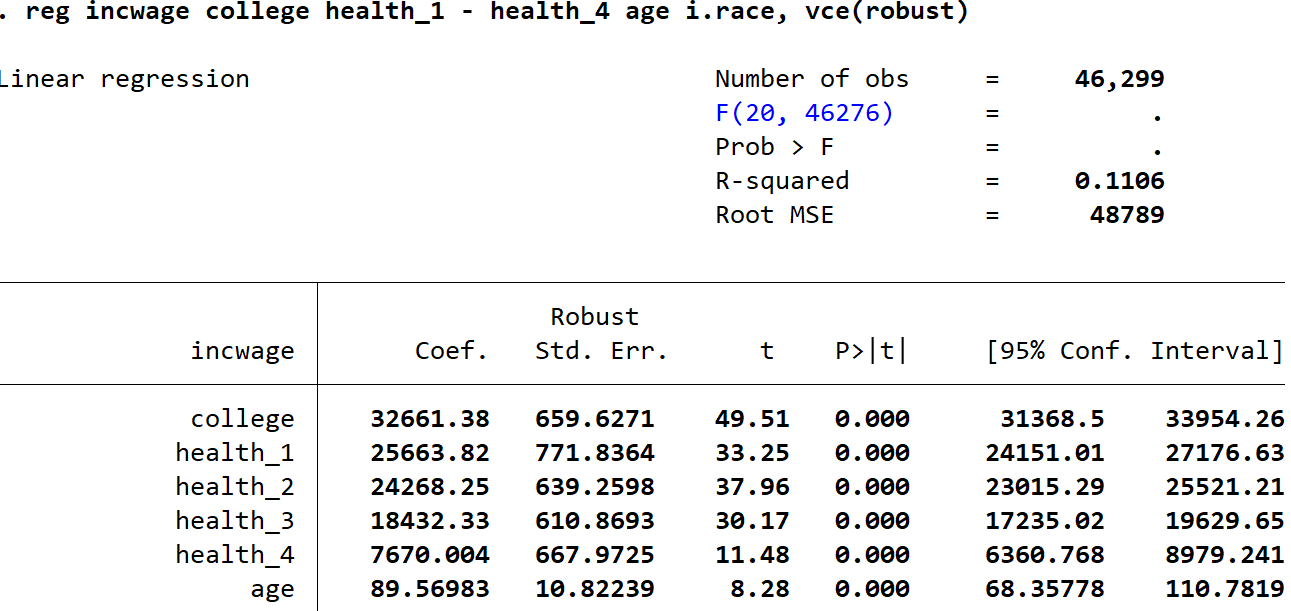
\includegraphics[width=0.9\textwidth]{figure/reg_est_f1.png}
		
		
\end{frame}



\begin{frame}[fragile]{Understanding the Frisch-Waugh-Lovell Theorem}
	
		
\begin{lstlisting}
reg college health_1 - health_4 age i.race, vce(robust)
predict college_rid, residuals

reg incwage college health_1 - health_4 age i.race, vce(robust)
reg incwage college_rid, vce(robust)
\end{lstlisting}
		
		\vspace{0.2cm}
		
	\begin{itemize}
		\item Regress \texttt{college} on all other covariates to obtain residuals \texttt{college\_rid}
		
		\vspace{0.2cm}
			\begin{itemize}
		\item \texttt{college\_rid} represents the part of \texttt{college} that is unrelated to other covariates
			\end{itemize}
		\vspace{0.2cm}
		
		\item Regress \texttt{incwage} on \texttt{college} and other covariates 
		
		\vspace{0.2cm}
		
		\item Regress \texttt{incwage} on \texttt{college\_rid} gives same coefficient as previous regression
		
	\end{itemize}
	
\end{frame}







\begin{frame}[fragile]{Understanding the Frisch-Waugh-Lovell Theorem}{Output}
		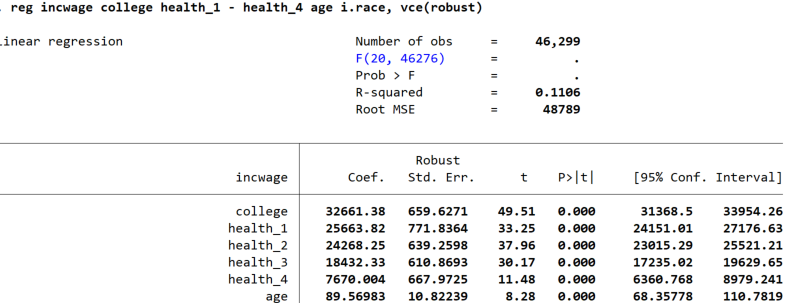
\includegraphics[width=0.9\textwidth]{figure/reg_est_f3.png}
		
		
\end{frame}



\begin{frame}[fragile]{Understanding the Frisch-Waugh-Lovell Theorem}{Output}
		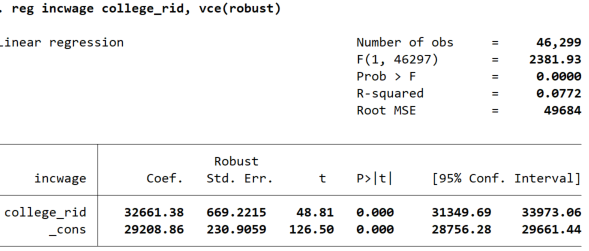
\includegraphics[width=0.9\textwidth]{figure/reg_est_f4.png}
		
		
\end{frame}

\begin{frame}[fragile]{Subgroup Analysis}

\begin{lstlisting}
reg incwage college i.health age year i.race if sex==1, vce(robust)
\end{lstlisting}
	\vspace{0.2cm}
\begin{itemize}
\item Option \textbf{if}: restrict sample to specific subgroup



\end{itemize}
\end{frame}

\begin{frame}[fragile]{Subgroup Analysis}{Output}
		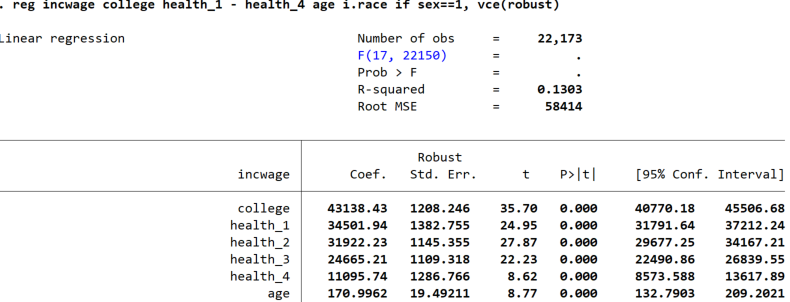
\includegraphics[width=0.9\textwidth]{figure/reg_est_f5.png}
		
		
\end{frame}

\begin{frame}[fragile]{Subgroup Analysis}
		
\begin{lstlisting}
reg incwage college gender college_gender i.health age year i.race, vce(robust)
\end{lstlisting}
		\vspace{0.2cm}
	\begin{itemize}
		\item Examine differential effect of \texttt{college} by gender 
		
		
		
	\end{itemize}
\end{frame}












\title[]  
{R Example}


\author 
{}

%\institute{Institute of Economics, Academia Sinica  \\ Econ, NTU}
%\institute{Institute of Economics, Academia Sinica  \\ IMES/IDAS, NCCU}
\institute{}

%\author 
%{楊子霆 \\ 中研院經濟所}

%\institute 
%{中正大學國際經濟專題研討}




\date
{}


\begin{frame}{}
	\titlepage
\end{frame}






\begin{frame}{R Example}{}
	\begin{itemize}
		\item See \textbf{regression.R}
		\vspace{0.2cm}
		\item Use cps\_2014\_16.dta
		\vspace{0.2cm}
		
	\end{itemize}
\end{frame}


\begin{frame}[fragile]{Examine Data}{skim(): Check for Missing Values}
		\begin{lstlisting}
# Load the skimr package
library(skimr)
			
# Check for missing values with skim()
skim(acs_2015)
\end{lstlisting}
		\vspace{0.2cm}
	\begin{itemize}
		\item \textbf{skim()} from the \textbf{skimr} package provides a comprehensive data summary
		\vspace{0.2cm}
		\item The function automatically reports:
		\vspace{0.2cm}
		\begin{itemize}
			\item Number of missing values for each variable
			\vspace{0.2cm}
			\item Proportion of missing data
			\vspace{0.2cm}
			\item Data type information and summary statistics
		\end{itemize}
		\vspace{0.2cm}
		\item More efficient than manually checking with \textbf{is.na()} or \textbf{complete.cases()}
	\end{itemize}
\end{frame}

\begin{frame}[fragile]{Create Sample for Analysis}{Create new variables}
\begin{lstlisting}
# Create a dummy variable for college education
acs_2015$college <- ifelse(acs_2015$educ99 >= 15, 1, 0)

# Create new gender variable (1 for male, 0 for female)
acs_2015$gender <- ifelse(acs_2015$sex == 1, 1, 0)
\end{lstlisting}
		\vspace{0.2cm}
	\begin{itemize}
		\item \texttt{ifelse()} function: 
				\vspace{0.2cm}
		\begin{itemize}
			\item Syntax: \texttt{ifelse(condition, value\_if\_true, value\_if\_false)}
					\vspace{0.2cm}
			\item Creates a new variable based on a condition
		\end{itemize}
	
	\end{itemize}
\end{frame}

\begin{frame}[fragile]{Create Sample for Analysis}{Create new variables}
\begin{lstlisting}
# Replace missing income wage values and remove NA rows
acs_2015$incwage[acs_2015$incwage == 9999999] <- NA
acs_2015 <- na.omit(acs_2015, cols = "incwage")

# Generate log of incwage
acs_2015$log_incwage <- log(acs_2015$incwage)
\end{lstlisting}
		\vspace{0.2cm}
	\begin{itemize}
		\item Handle missing values in \texttt{incwage}:
				\vspace{0.2cm}
		\begin{itemize}
			\item Replace 9999999 (missing value code) with \texttt{NA}
					\vspace{0.2cm}
			\item \texttt{na.omit()} removes rows with \texttt{NA} in \texttt{incwage}
					\vspace{0.2cm}
		\end{itemize}
		\item Create log-transformed income variable:
				\vspace{0.2cm}
		\begin{itemize}
			\item \texttt{log()} function calculates natural logarithm
					\vspace{0.2cm}
			\item Useful for analyzing proportional effects and normalizing skewed distributions
		\end{itemize}
	\end{itemize}
\end{frame}



\begin{frame}[fragile]{Create Sample for Analysis}{mutate(): Create new variables}
\begin{lstlisting}
# Generate health dummy variables using dplyr
acs_2015 <- acs_2015 %>%
mutate(
health_1 = as.integer(health == 1),
health_2 = as.integer(health == 2),
health_3 = as.integer(health == 3),
health_4 = as.integer(health == 4),
health_5 = as.integer(health == 5)
)
\end{lstlisting}
		\vspace{0.2cm}
	\begin{itemize}
		\item Use \texttt{dplyr}'s \textbf{mutate()} function to create all dummy variables in one step
		\vspace{0.2cm}
			\begin{itemize}
		\item The \texttt{\%>\%} pipe operator makes the code more readable by passing data through operations
		\vspace{0.2cm}
		\item \textbf{as.integer()} converts logical values to 0 or 1
		\vspace{0.2cm}
			\end{itemize}
		\item More explicit approach that clearly shows all variables being created
	\end{itemize}
\end{frame}



%\begin{frame}[fragile]{Create Sample for Analysis}{Use loop to create dummy variables}
%	\begin{itemize}
%\begin{lstlisting}
%# Generate health dummy variables
%for (i in 1:5) {
%acs_2015[[paste0("health_", i)]] <- 
%as.integer(acs_2015$health == i)
%}
%\end{lstlisting}
%		\vspace{0.2cm}
%		\item Use a \texttt{for} loop to create binary variables \texttt{health\_1}, \texttt{health\_2}, ..., \texttt{health\_5}
%						\vspace{0.2cm}
%		\item \textbf{as.integer()} converts logical values to 0 or 1
%						\vspace{0.2cm}
%		\item The loop generates 5 binary variables capturing different values of the \texttt{health} variable
%	\end{itemize}
%\end{frame}


\begin{frame}[fragile]{R Command: lm\_robust()}
	\begin{itemize}
		\item \texttt{lm\_robust()}: Linear Models with Robust Standard Errors in R
		\vspace{0.2cm}
		\item Syntax:
		\vspace{0.2cm}
\begin{lstlisting}
lm_robust(formula, data, subset, weights, se_type, ...)
\end{lstlisting}
		\item Required package:
\begin{lstlisting}
library(estimatr)
\end{lstlisting}
	\end{itemize}
\end{frame}

\begin{frame}[fragile]{Reducing OVB by including covariates}
\begin{lstlisting}
# Define your models with robust standard errors
model1 <- lm_robust(incwage ~ college, data = acs_2015, se_type = "HC1")
model2 <- lm_robust(incwage ~ college + age + health_1 + health_2 + health_3 + health_4, data = acs_2015, se_type = "HC1")

# Print summaries to get robust standard errors
summary(model1)
summary(model2)
\end{lstlisting}
		\vspace{0.2cm}
	\begin{itemize}
		\item Regress \texttt{incwage} on \texttt{college} using robust standard errors
		\vspace{0.2cm}
		\item Use \textbf{lm\_robust()} with \textbf{se\_type = "HC1"} for direct computation of robust standard errors
	\end{itemize}
\end{frame}

\begin{frame}[fragile]{Subgroup Analysis}
\begin{lstlisting}
model3 <- lm_robust(incwage ~ college + age + factor(race) + health_1 + health_2 + health_3 + health_4, data = acs_2015, subset = (gender == 1), se_type = "HC1")

# Print summary to get robust standard errors
summary(model3)
\end{lstlisting}
		\vspace{0.2cm}
	\begin{itemize}
		\item \texttt{subset} parameter in \textbf{lm\_robust()}:
		\vspace{0.2cm}
		\begin{itemize}
			\item Allows you to specify a condition for selecting observations
			\vspace{0.2cm}
			\item In this case, \textbf{subset = (gender == 1)} selects only male observations
			\vspace{0.2cm}
			\item Equivalent to filtering the data before running the regression
		\end{itemize}
		
	\end{itemize}
\end{frame}

\begin{frame}[fragile]{Subgroup Analysis}
\begin{lstlisting}
# Create interaction term
acs_2015$college_gender <- acs_2015$college * acs_2015$gender

# Define the model with interaction term and robust standard errors
model_interaction <- lm_robust(incwage ~ college + gender + college_gender + 
health_1 + health_2 + health_3 + health_4 + 
age + factor(race), data = acs_2015, se_type = "HC1")

# Print summary to get robust standard errors
summary(model_interaction)
\end{lstlisting}
		\vspace{0.2cm}
	\begin{itemize}
		\item Create an interaction term between \texttt{college} and \texttt{gender}
		\vspace{0.2cm}
		\item Include the interaction term in the regression model with robust standard errors
	\end{itemize}
\end{frame}


\begin{frame}{Suggested Readings}
	\begin{itemize} 
		\item Chapter 2, Mastering Metrics: The Path from Cause to Effect
		\vspace{0.2cm}
		\item Chapter 3, Mostly Harmless Econometrics
		\vspace{0.2cm}
		\item Chapter 2, Causal Inference: The Mixtape
	\end{itemize}
\end{frame}




\end{document} 
